\documentclass[12pt,letterpaper]{report}
\usepackage[margin=1in]{geometry}
\usepackage{graphicx}
\usepackage{amsmath}
\usepackage[font=small,labelfont=bf]{caption}
\usepackage[justification=centering]{caption}
\usepackage{tikz}
\usepackage{circuitikz}
\usepackage{siunitx}
\usepackage{float}
\newlength \figwidth
\setlength \figwidth {0.75\linewidth}

\begin{document}

\title{E153 Laboratory Assignment \#4}
\author{Courtney Keeler and Stephen Pinto\\
Harvey Mudd College}
\date{October 21, 2013}
\maketitle

\section*{List of Materials}
\begin{itemize}
	\item Tektronix 2212 Oscilloscope
	\item Pomona 4550B (10X probe)
	\item Elenco LCM-1950 Multimeter
	\item Lab Station 7 Transformer (s.n. 139 01 665)
	\item 2.2 kOhm resistor
	\item Electrolytic capacitors (10 $\mu$F, 3.3 $\mu$F, 100 $\mu$F, and .47 $\mu$F)
\end{itemize}

\section*{Purpose}
The purpose of this lab is to build transformer circuits and do neat things with them.

\section*{3.2 Half-Wave Rectifier}
\subsection*{Procedure}

\begin{enumerate}
\item Construct the circuit shown in Figure \ref{fig:circuit_1}
\item To zero the scope to the transformer, turn the transformer off, leaving the probe across the resistor, and match the cursor to the signal (should be flat line)
\item Measure the voltage across just the diode to find the voltage drop across the diode
\item Measure just the voltage out of the transformer to see the original peak voltage
\item Measure the voltage across the resistor with the full circuit intact to see the final peak voltage
\item Compare the original and final peak voltage values
\end{enumerate}

\begin{figure}[H]
\centering
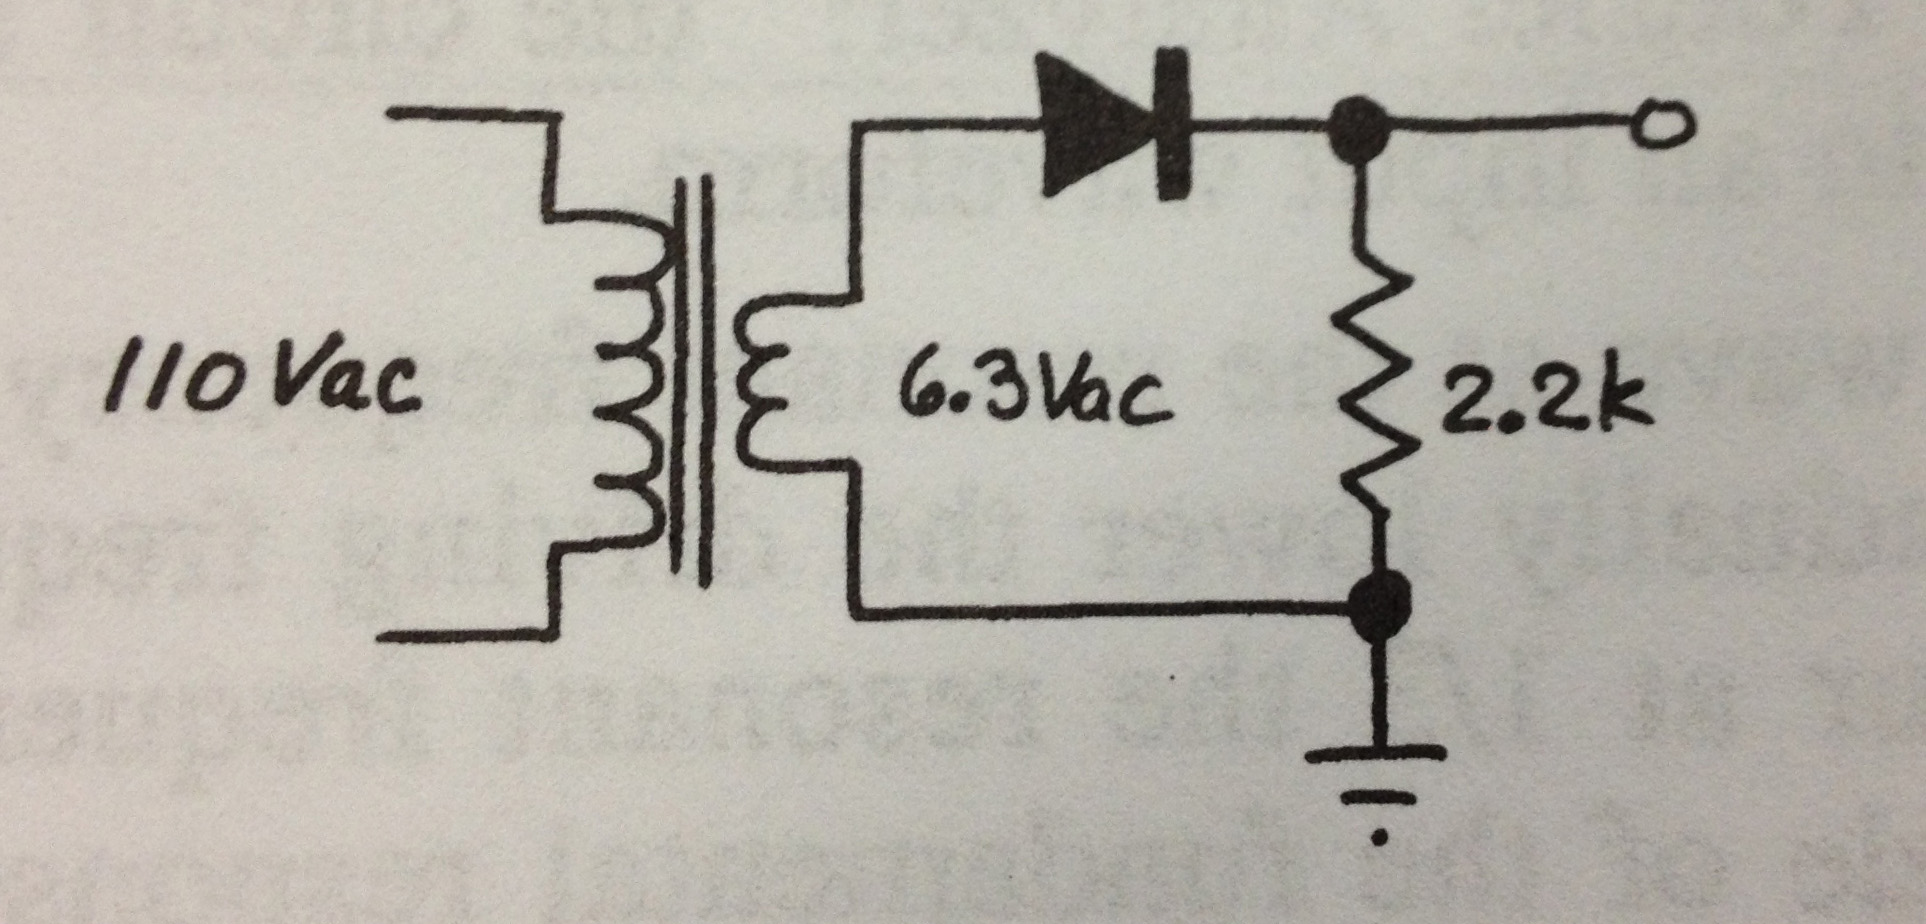
\includegraphics[width=\figwidth, keepaspectratio=true]{lab4/circuit_1.jpg}
\caption{Circuit configuration for the half-wave rectifier. The diode is a 1N4001.}
\label{fig:circuit_1}
\end{figure}

\subsection*{Results}

Voltage across diode: 0.7 V.

\begin{figure}[H]
\centering
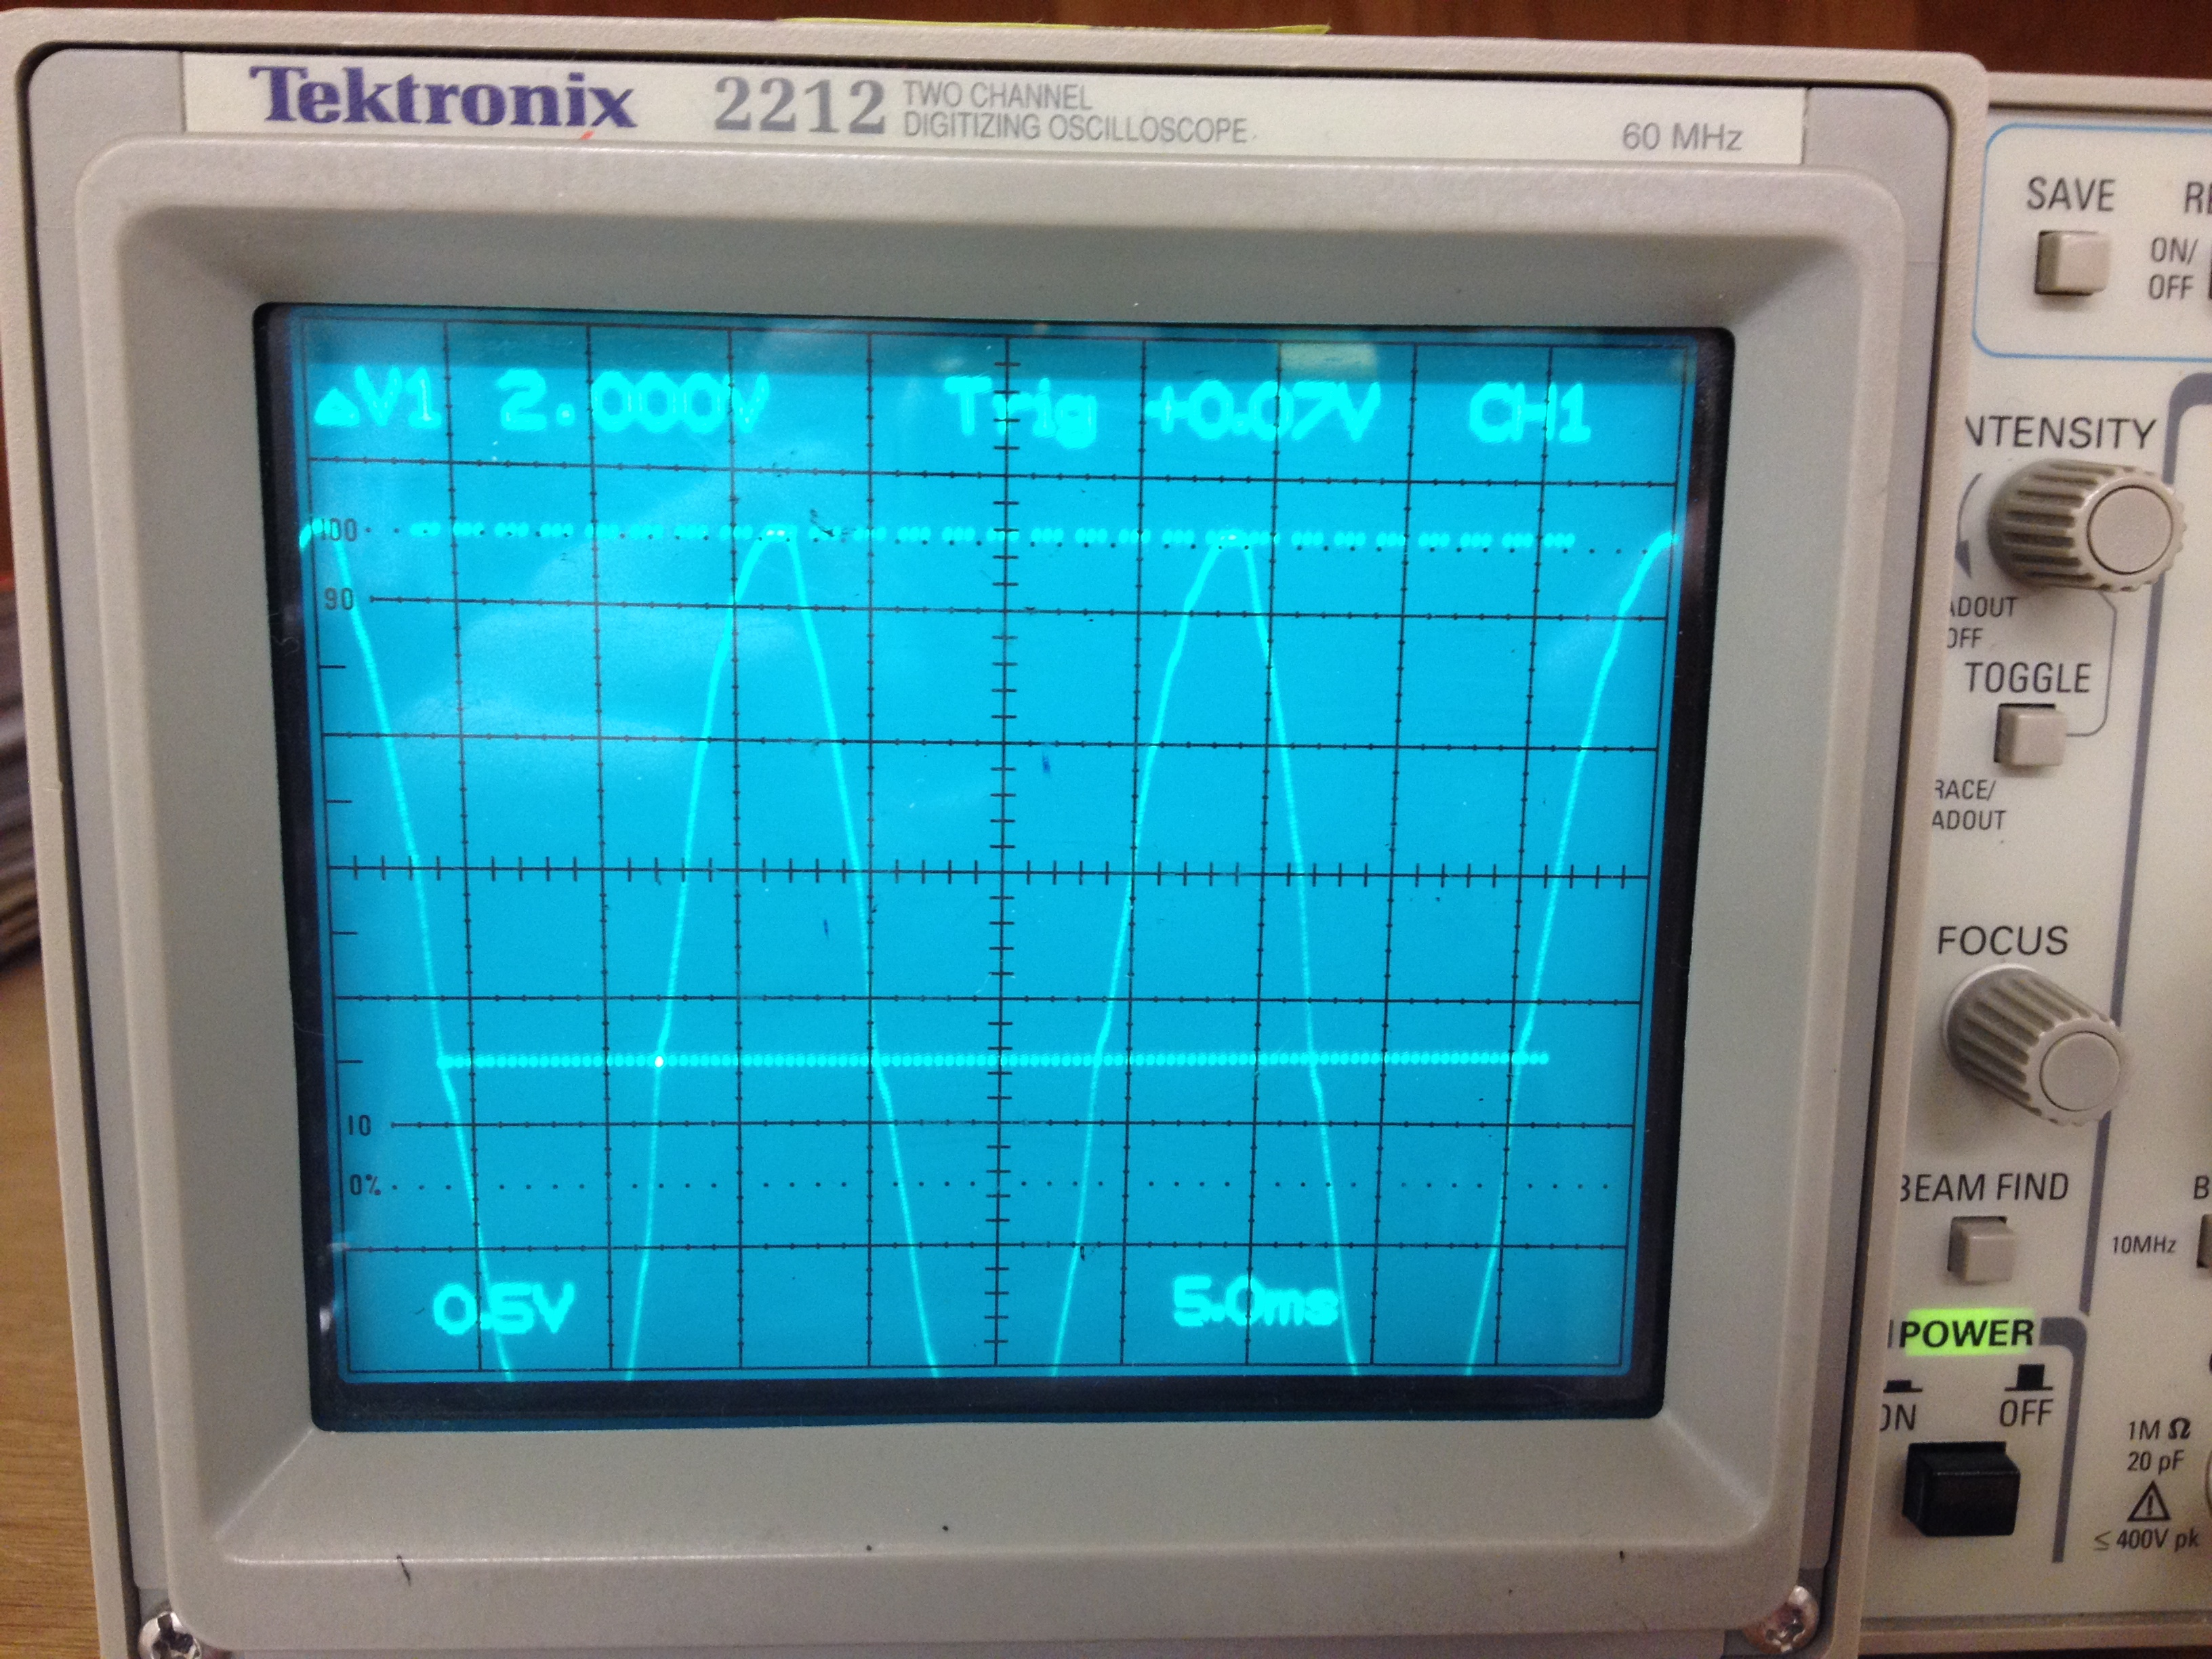
\includegraphics[width=\figwidth, keepaspectratio=true]{lab4/3_2_transformer.jpg}
\caption{Output waveform of the voltage out of the transistor.}
\label{fig:3.2_transformer}
\end{figure}

\begin{figure}[H]
\centering
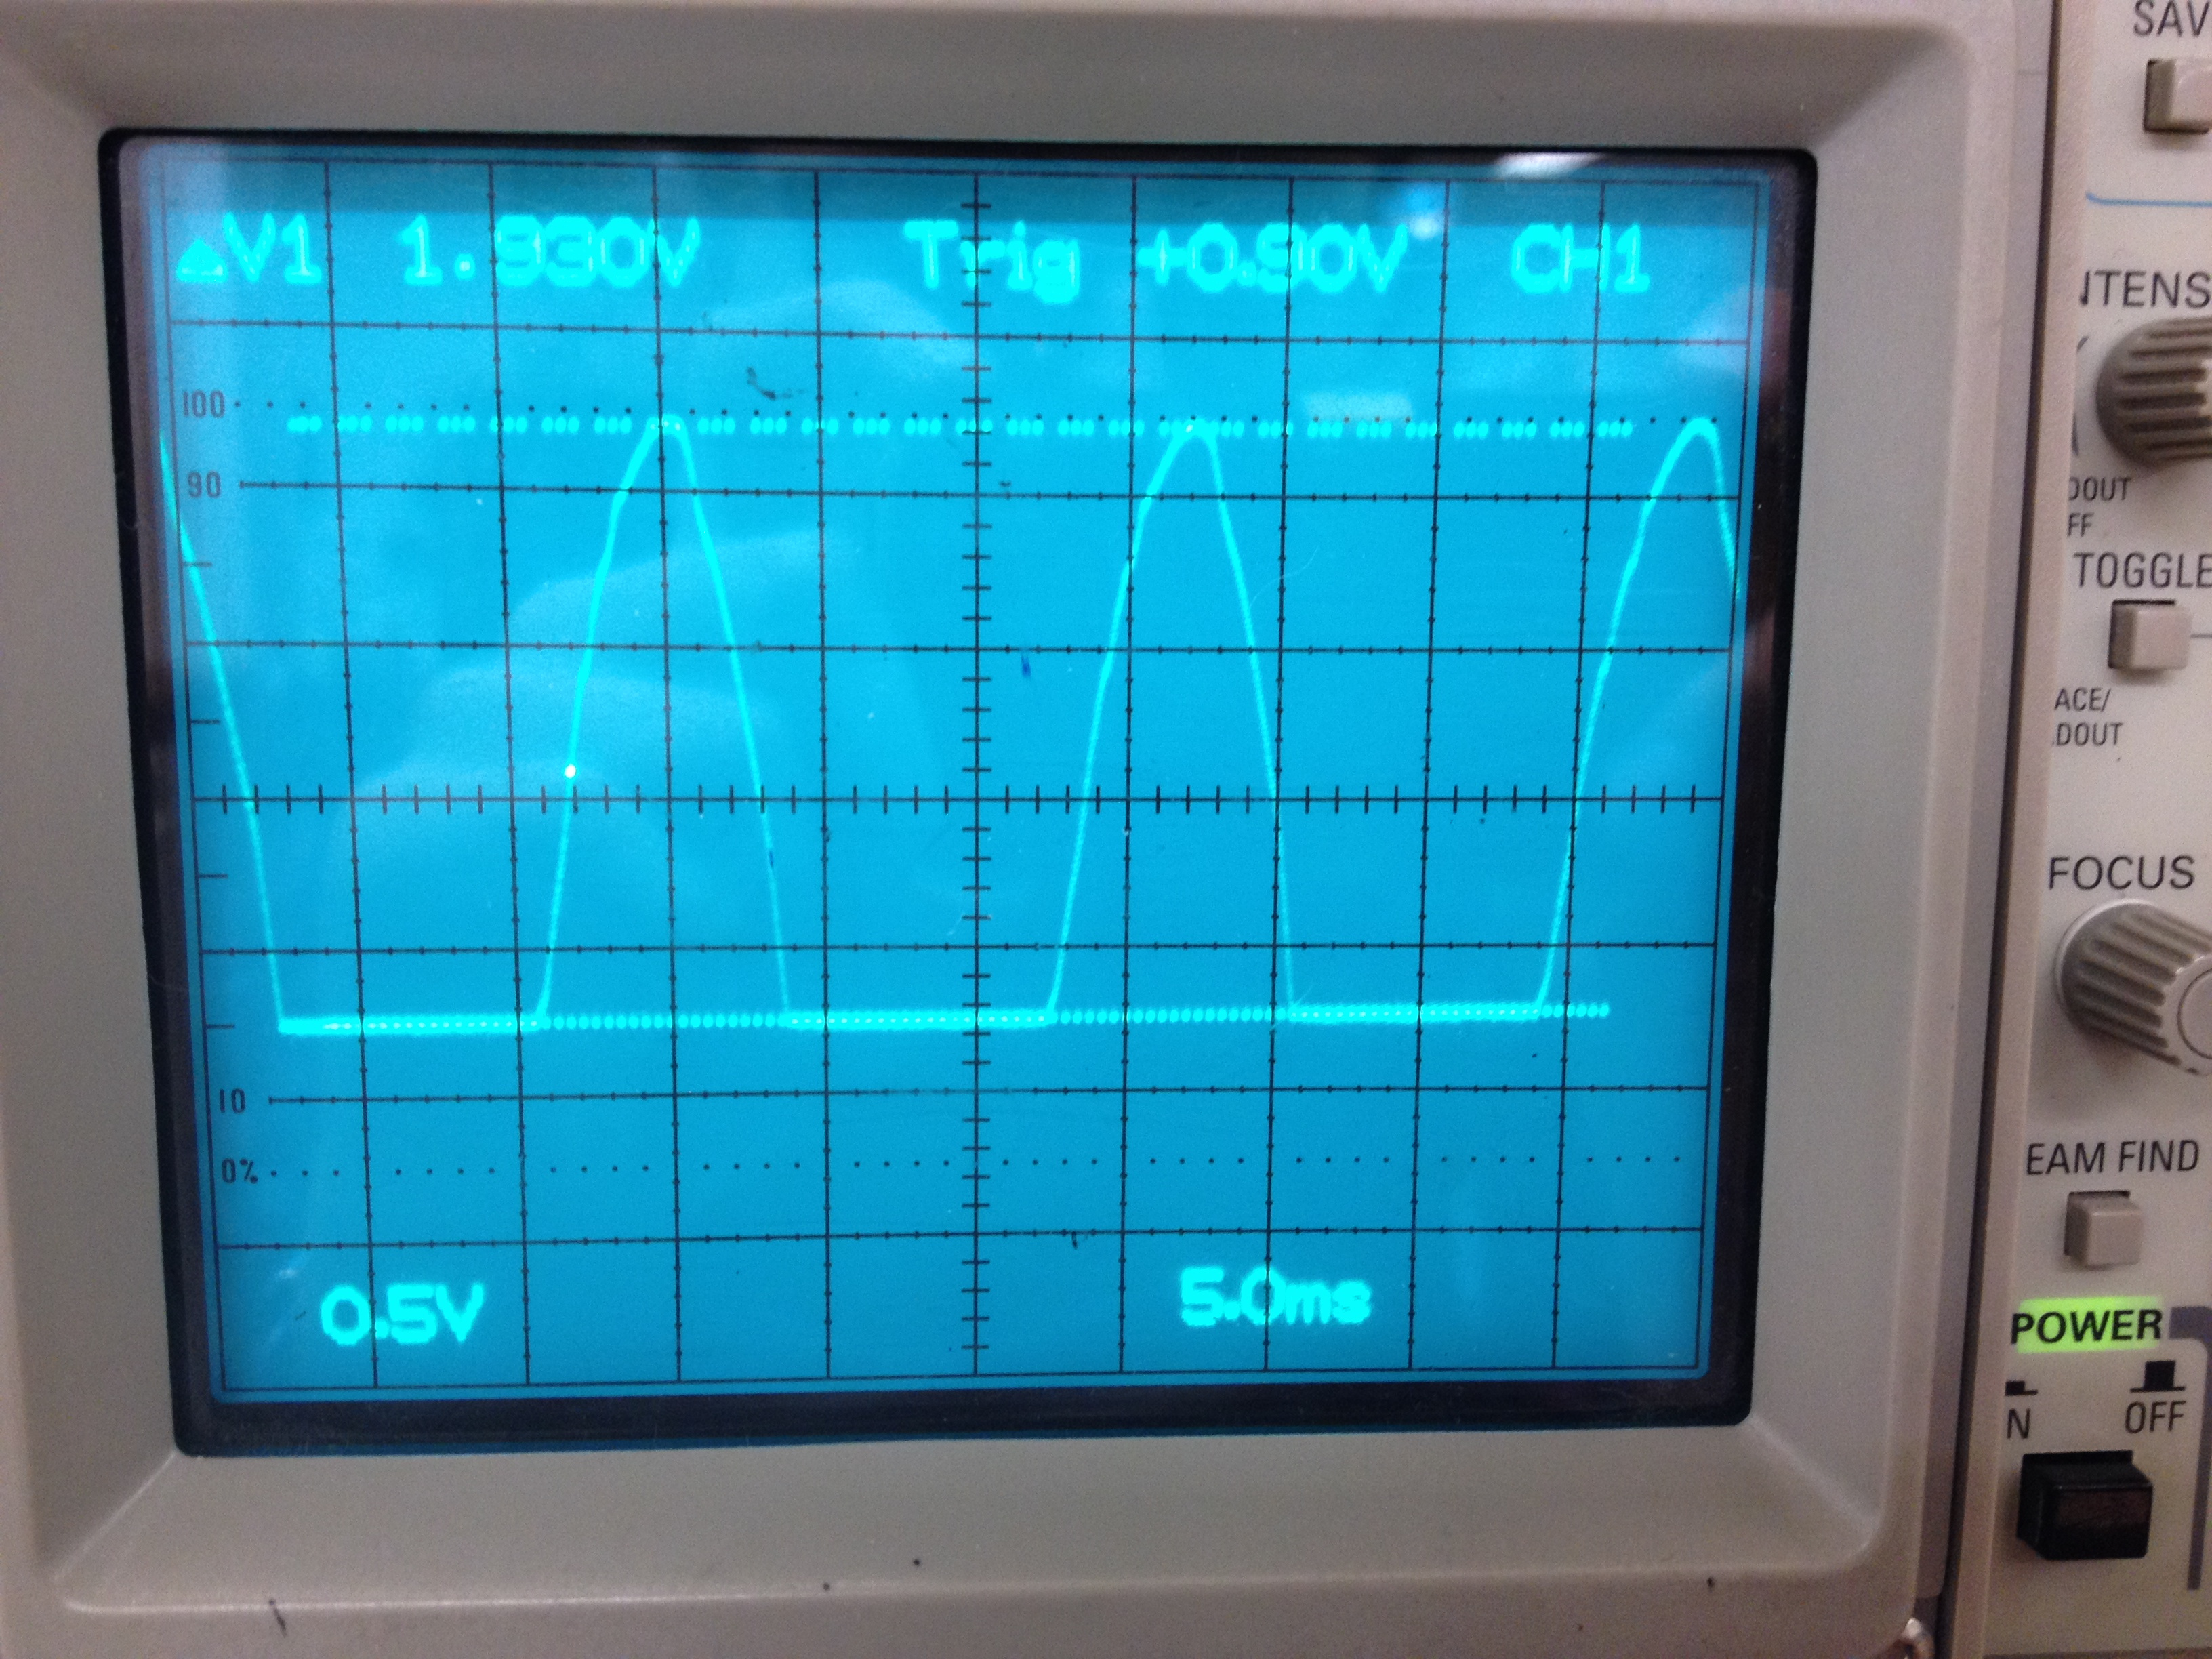
\includegraphics[width=\figwidth, keepaspectratio=true]{lab4/3_2_resistor_final.jpg}
\caption{Output waveform of the voltage across the resistor in the final half-wave rectifier circuit configuration.}
\label{fig:3.2_resistor_final}
\end{figure}

\subsection*{Analysis}

The waveform shown in Figure 
\ref{fig:3.2_resistor_final}
 is what is expected. It is a half wave rectifier, so we expect to see only the positive half of the input sin wave from the transistor (shown in Figure \ref{fig:3.2_transformer}). The frequency of both signals remains at 60 Hz. However, the peak voltage straight out of the transformer is 20.00V, and when we construct the full half-wave rectifier circuit the peak voltage is 19.3 V. This drop in voltage is due to the voltage drop across the diode, which we measured as 0.7 V and we can verify by
$$
V_D = 20-19.3=0.7\text{ V}.\footnote{the figures above show values that are ten times less than the values used here. However, recall that when measuring with a 10X probe, the measured values must be multiplied by 10.}
$$

Since this circuit is a half-wave (not full-wave) rectifier, it only works on one polarity of input voltage. This is to say that on the forward bias (i.e. when the input voltage is greater than zero) there is a positive output of the circuit, and on the reverse bias,  there is an output of zero from the circuit.

\section*{3.3 Full-Wave Bridge Rectifier}
\subsection*{Procedure}

\begin{enumerate}
\item Construct the circuit shown in Figure \ref{fig:circuit_2}
\item To zero the scope to the transformer, turn the transformer off, leaving the probe across the resistor, and match the cursor to the signal (should be flat line)
\item View the output waveform using the 10X probe and oscilloscope
\item Look at the near-zero regions and measure the duration of the flat regions
\end{enumerate}

\begin{figure}[H]
\centering
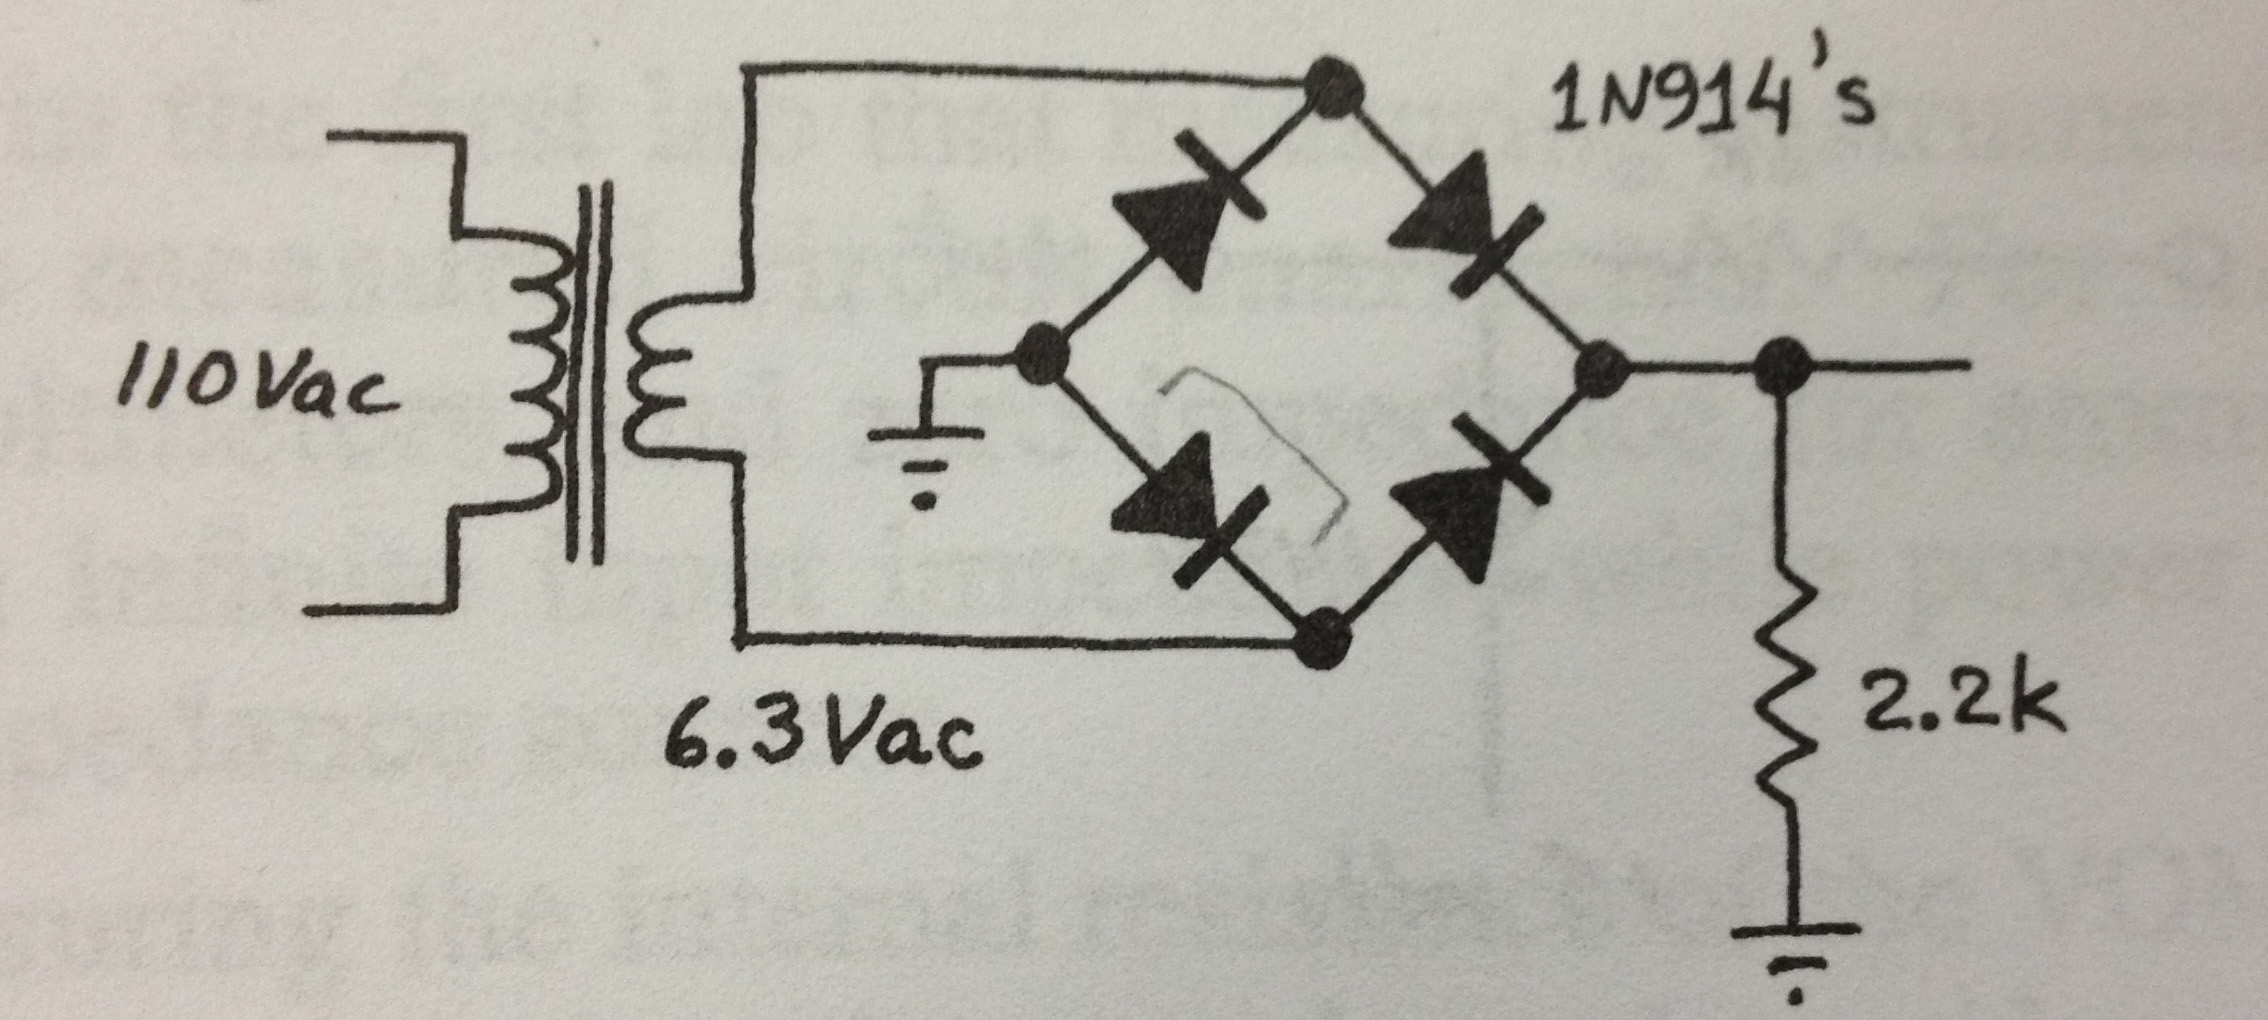
\includegraphics[width=\figwidth, keepaspectratio=true]{lab4/circuit_2.jpg}
\caption{Circuit configuration for the half-wave rectifier. The diodes are all 1N4001.}
\label{fig:circuit_2}
\end{figure}

\subsection*{Results}

\begin{figure}[H]
\centering
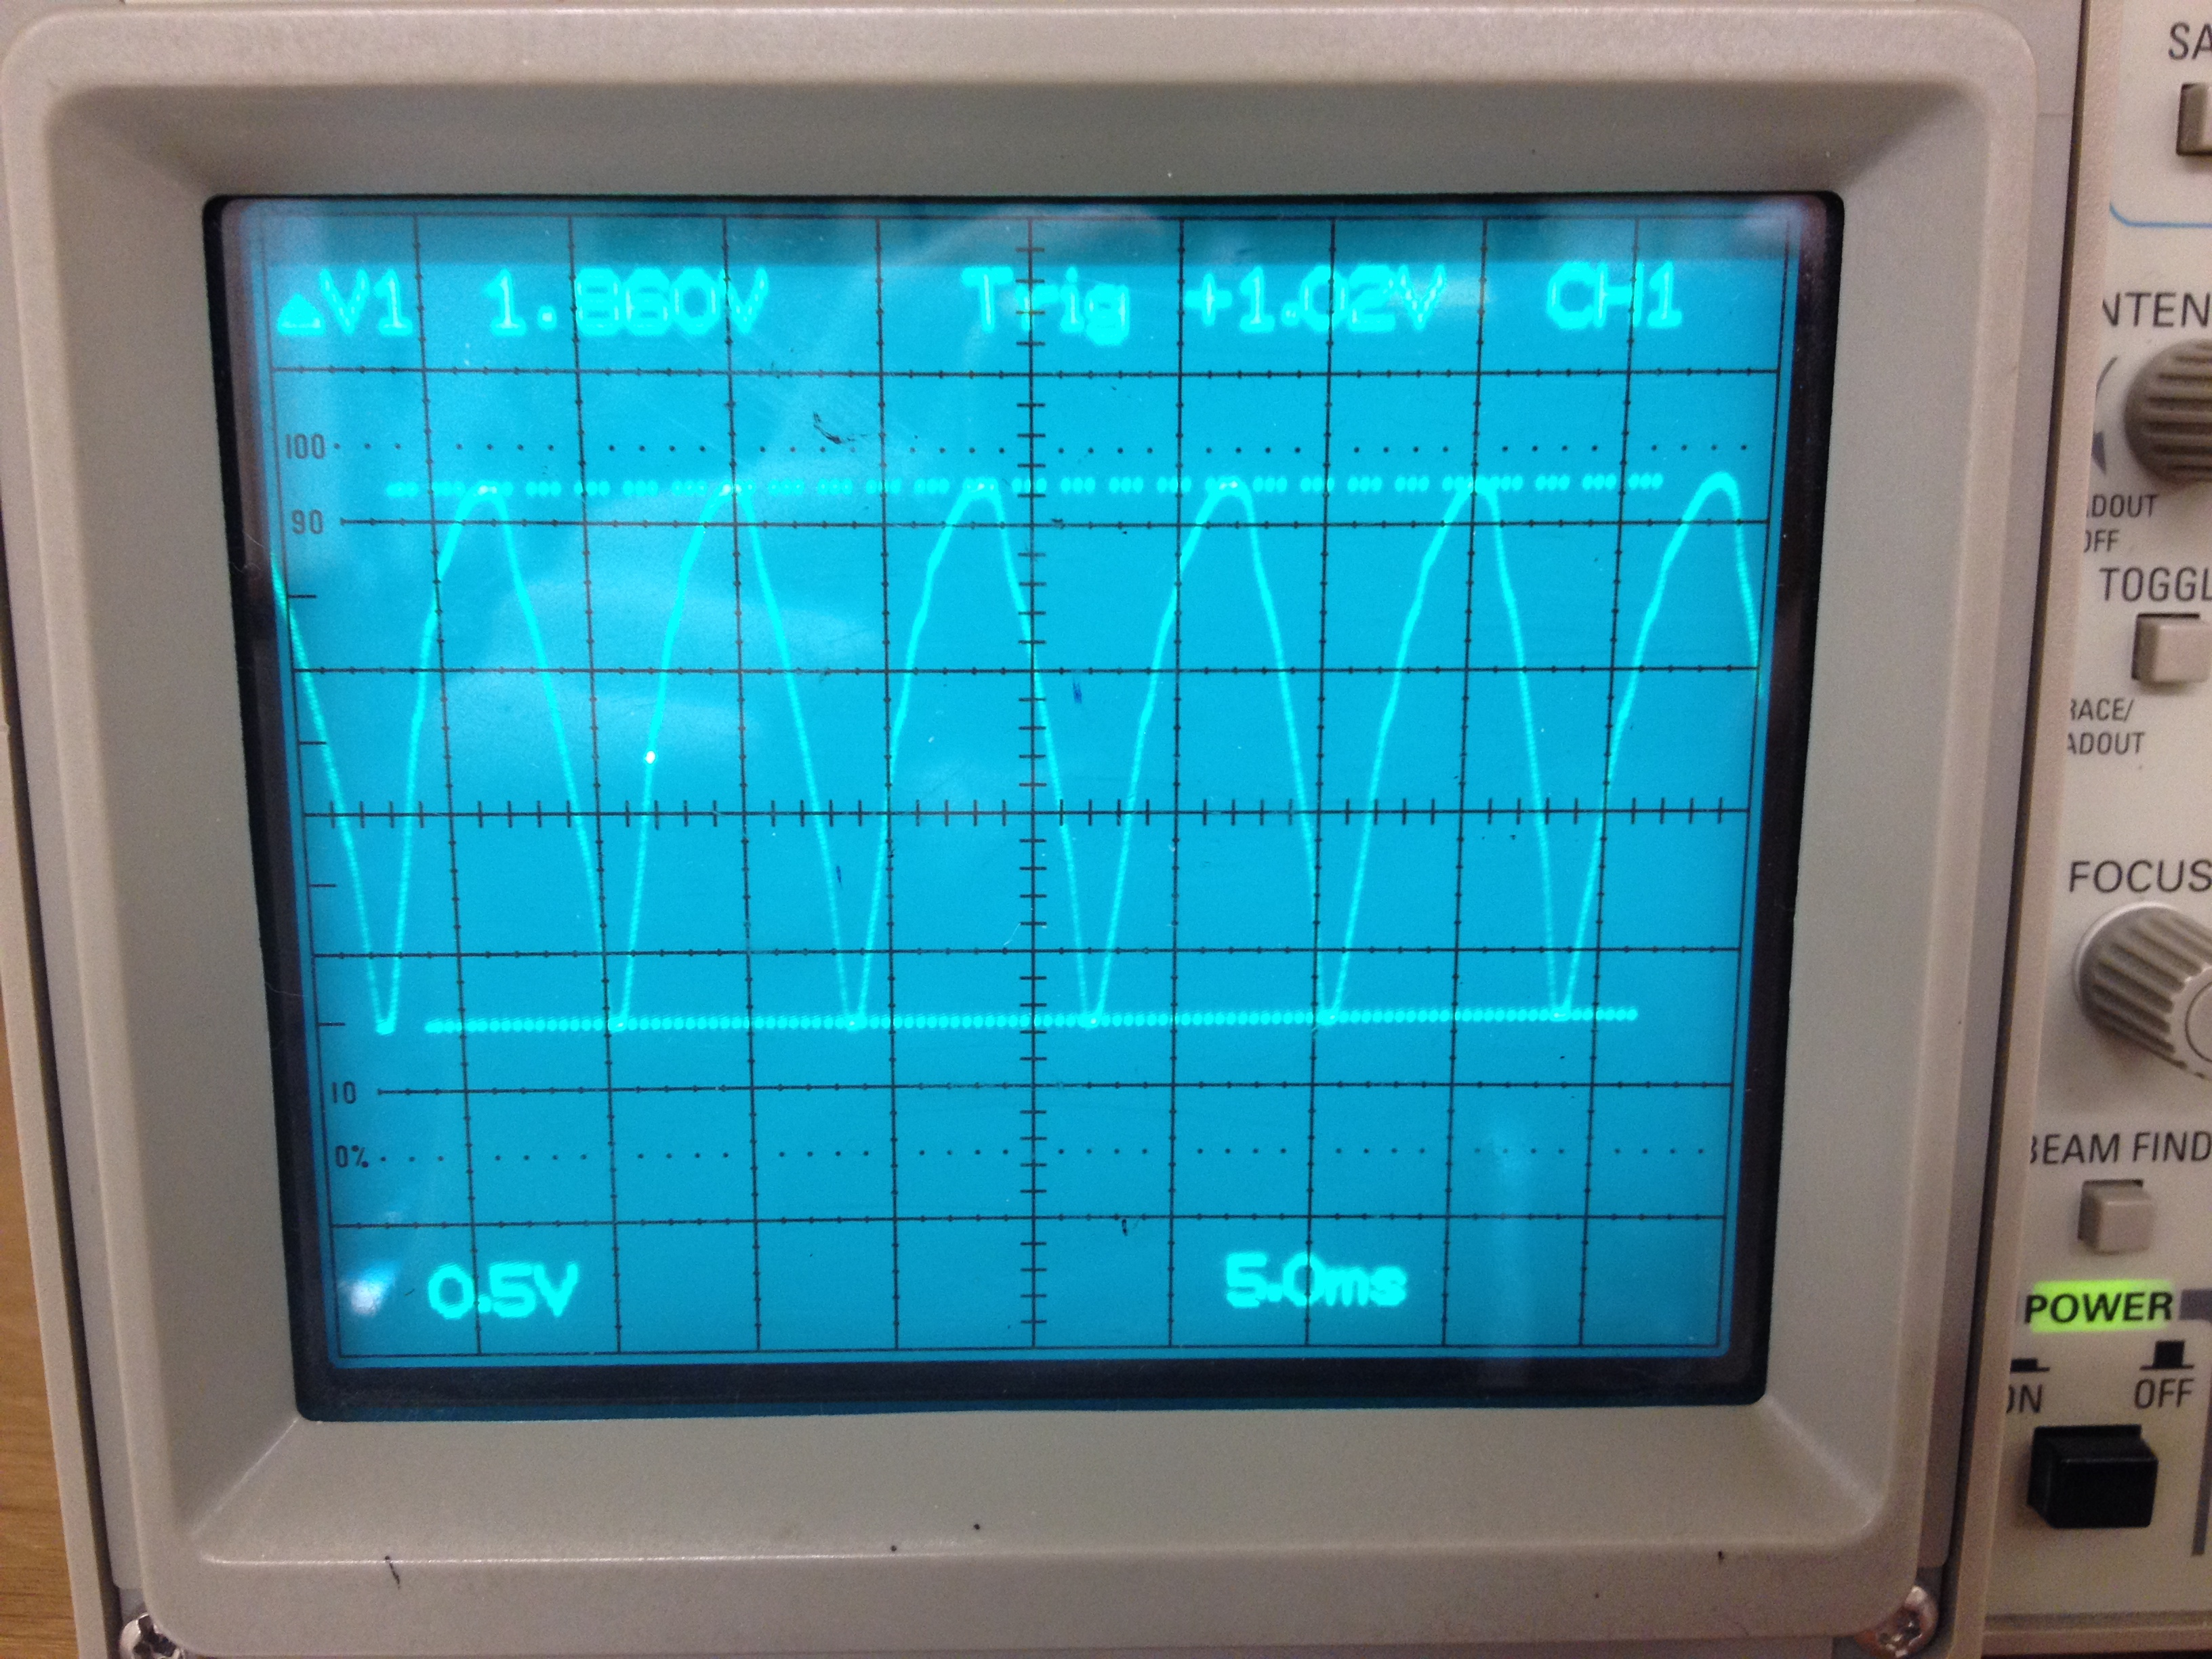
\includegraphics[width=\figwidth, keepaspectratio=true]{lab4/3_3_resistor.jpg}
\caption{Output waveform of the voltage across the resistor in the final full-wave rectifier circuit configuration.}
\label{fig:3.3_resistor}
\end{figure}

Flat region duration: 364.00 $\mu$s.

\subsection*{Analysis}

The peak voltage of the input sine wave from the transformer is still 20.00 V. There is now a greater drop in the output voltage peak. Figure \ref{fig:3.3_resistor} shows the output peak voltage to be 18.6 V, which is 1.4 V less than the input peak. This is to be expected, since there are now two diodes in the path of the current, meaning there will be two voltage drops of 0.7 V.

The Art of Electronics student manual asks what would happen if any one of the four diodes were to be reversed. In this case, ground would be forced at two places in the circuit, causing the circuit to become unstable and fail.

The reason for the flat regions near zero is due to the voltage being between 0 and 0.7 volts. At this time, the diode is taking all of the voltage drop. This is why in a simplified model, diodes are said to "turn on" at 0.7 V.

\section*{3.4 Ripple}
\subsection*{Procedure}

\begin{enumerate}
\item Construct the circuit shown in Figure %\ref{3.4_circuit}
\item View the output waveform on the oscilloscope
\item Zero the cursor
\item Measure Vr and Vm
\item Replace the capacitor with the remaining values, one at a time
\end{enumerate}

\subsection*{Results}

\begin{table}[ht]
\caption{Experimental Ripple Results} % title of Table
\centering 
    \begin{tabular}{| c | c | c | c | c |}
    \hline  
    C (uF) & Vr (V) & Vm (V) & $\Delta$ t & R (k$\Omega$) \\
    \hline
    10.4 & 14.23 & 18.6 & 6.1344 & 2.169 \\
    21.3 &16.10 & 18.6& 6.4406 & 2.169 \\
    3.128 & 9.69 & 18.6& 4.9656 &  2.169 \\
    10.4 & 10.98 &18.6& 5.1719 &.977 \\
    10.4 &14.42 & 18.6& 5.8625 & 2.363 \\
    10.4 &16.36 &18.6& 6.4719 & 4.608 \\
    \hline
    \end{tabular}
    \label{table:vpp}
\end{table}

%Experimental:
%C = 10.4 uF,  Vr = 14.23 V, Vm = 18.6, delta t = 6.1344 ms, R = 2.169 kOhms
%C = 21.3 uF, Vr = 16.10 V, Vm = 18.6, delta t = 6.4406 ms, R = 2.169 kOhms
%C = 3.128 uF, Vr = 9.69 V, Vm = 18.6, delta t = 4.9656 ms, R =  2.169 kOhms
%C = 10.4 uF,  Vr = 10.98 V, Vm = 18.6, delta t = 5.1719 ms, R = .977 kOhms
%C = 10.4 uF, Vr = 14.42 V, Vm = 18.6, delta t = 5.8625 ms, R = 2.363 kOhms
%C = 10.4 uF, Vr = 16.36 V, Vm = 18.6, delta t = 6.4719 ms, R = 4.608 kOhms

\subsection*{Analysis}

\subsection*{Calculations}
This is how to come up with an equation to find the capacitor value from the ripple voltage: Stephen's tiny red notebook

\section*{Transformers 3.7}
\subsection*{Procedure}

\begin{enumerate}
\item Construct the circuit shown in Figure \ref{fig:circuit_3}
\item View the output on the oscilloscope for a range of amplitudes of sin waves
\item Repeat the above step for square waves, then triangle waves
\item Add a 7805 three terminal voltage regulator to the power supply and record how much the  output voltage varies as the load changes from 1 mA to 50 mA
\end{enumerate}

\begin{figure}[H]
\centering
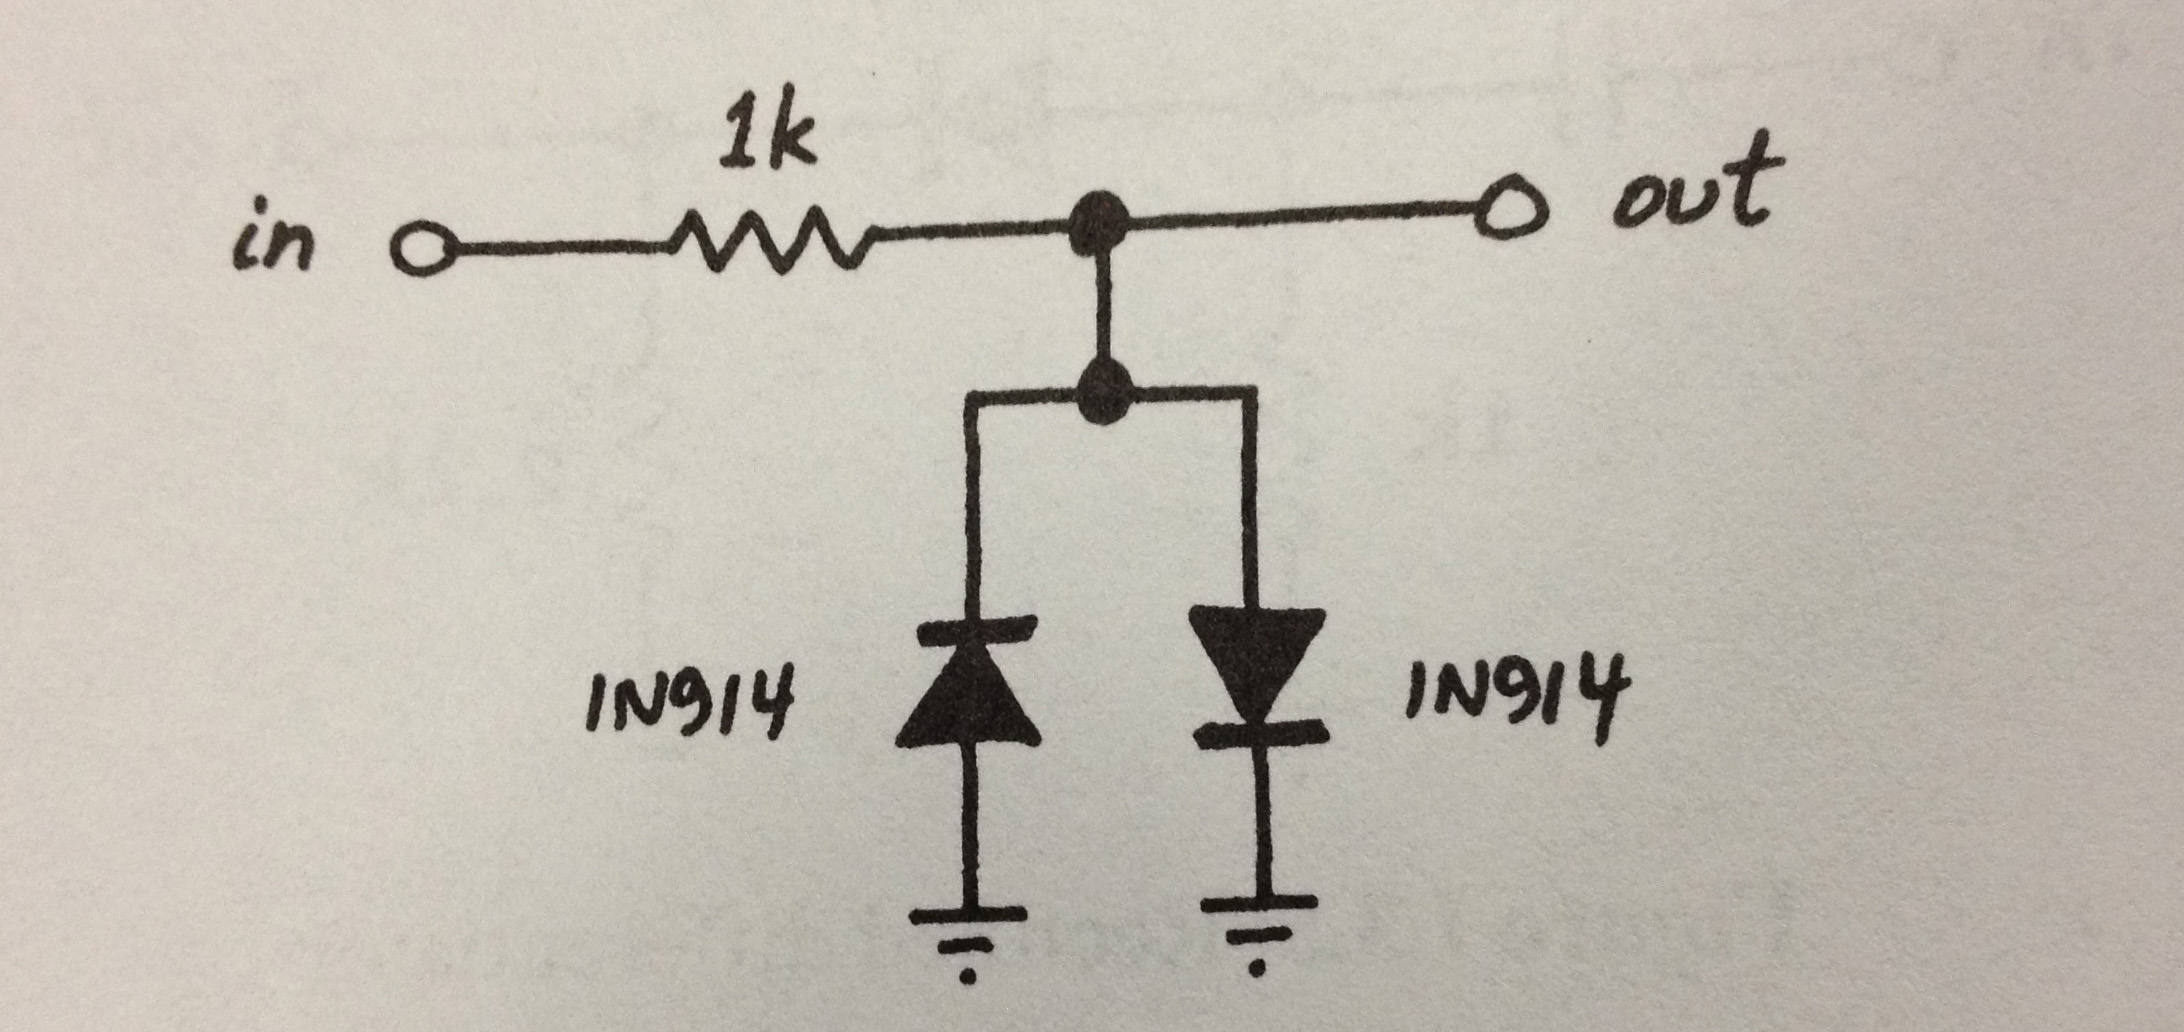
\includegraphics[width=\figwidth, keepaspectratio=true]{lab4/circuit_3.jpg}
\caption{Circuit configuration for the diode limiter. The diodes are all 1N4001.}
\label{fig:circuit_3}
\end{figure}

\subsection*{Results}

For a sin wave input, as the magnitude of the wave increases, the output magnitude also increases. However, it does so at a non-linear rate. The output peak output voltage is limited to 0.7 V and approaches it from below as the input magnitude increases. For this reason, the output for small input voltages resembles a sin wave, but as the input increases, the output begins to look like a square wave.

The higher the input voltage, the more current going through the resistor (and thus the diode), since only one diode is forward biased (i.e., on) at a time and takes the entirety of the current.

\begin{figure}[H]
\centering
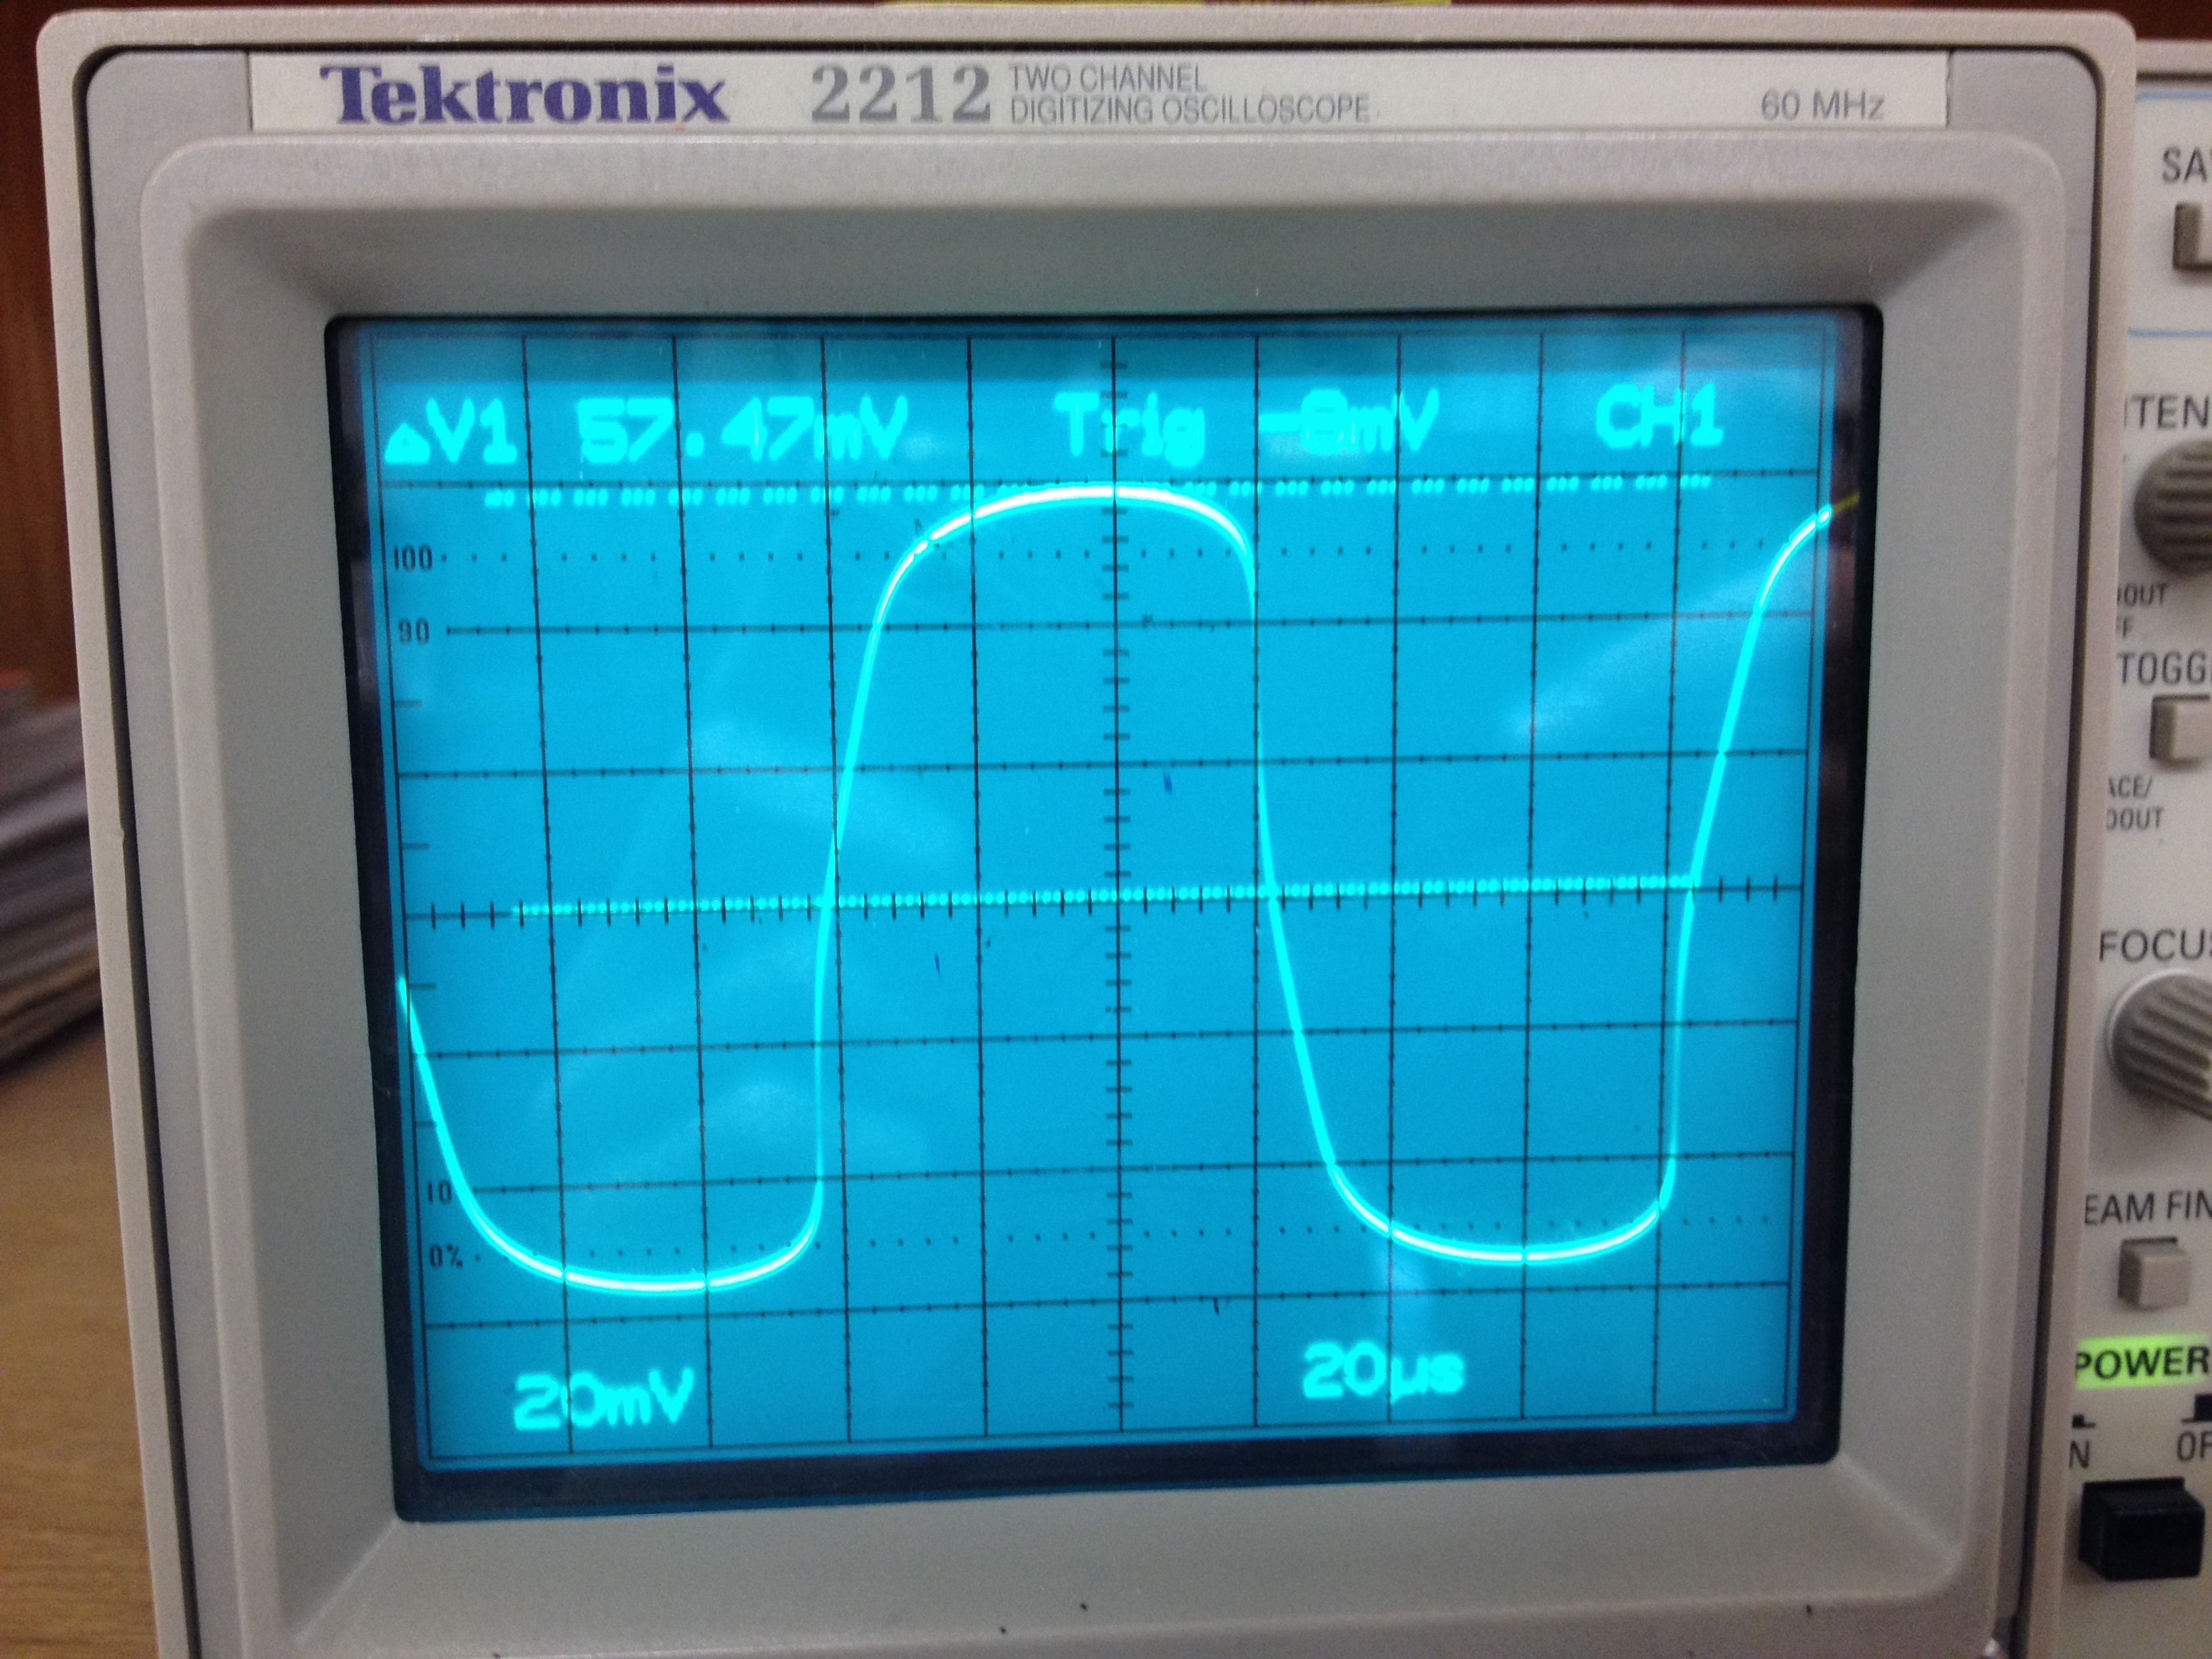
\includegraphics[width=\figwidth, keepaspectratio=true]{lab4/3_7_1.jpg}
\caption{Output waveform of the diode limiter when the input is a 2 $\text{V}_{\text{pp}}$ 8 kHz sine wave}
\label{fig:3_7_1}
\end{figure}

When the input is a square wave, the output behaves the same way, except instead of starting as a sin wave it starts looking like an attenuated square wave. As the input magnitude increases, the attentuation increases and the output voltage stops increasing at 0.7 V.

\begin{figure}[H]
\centering
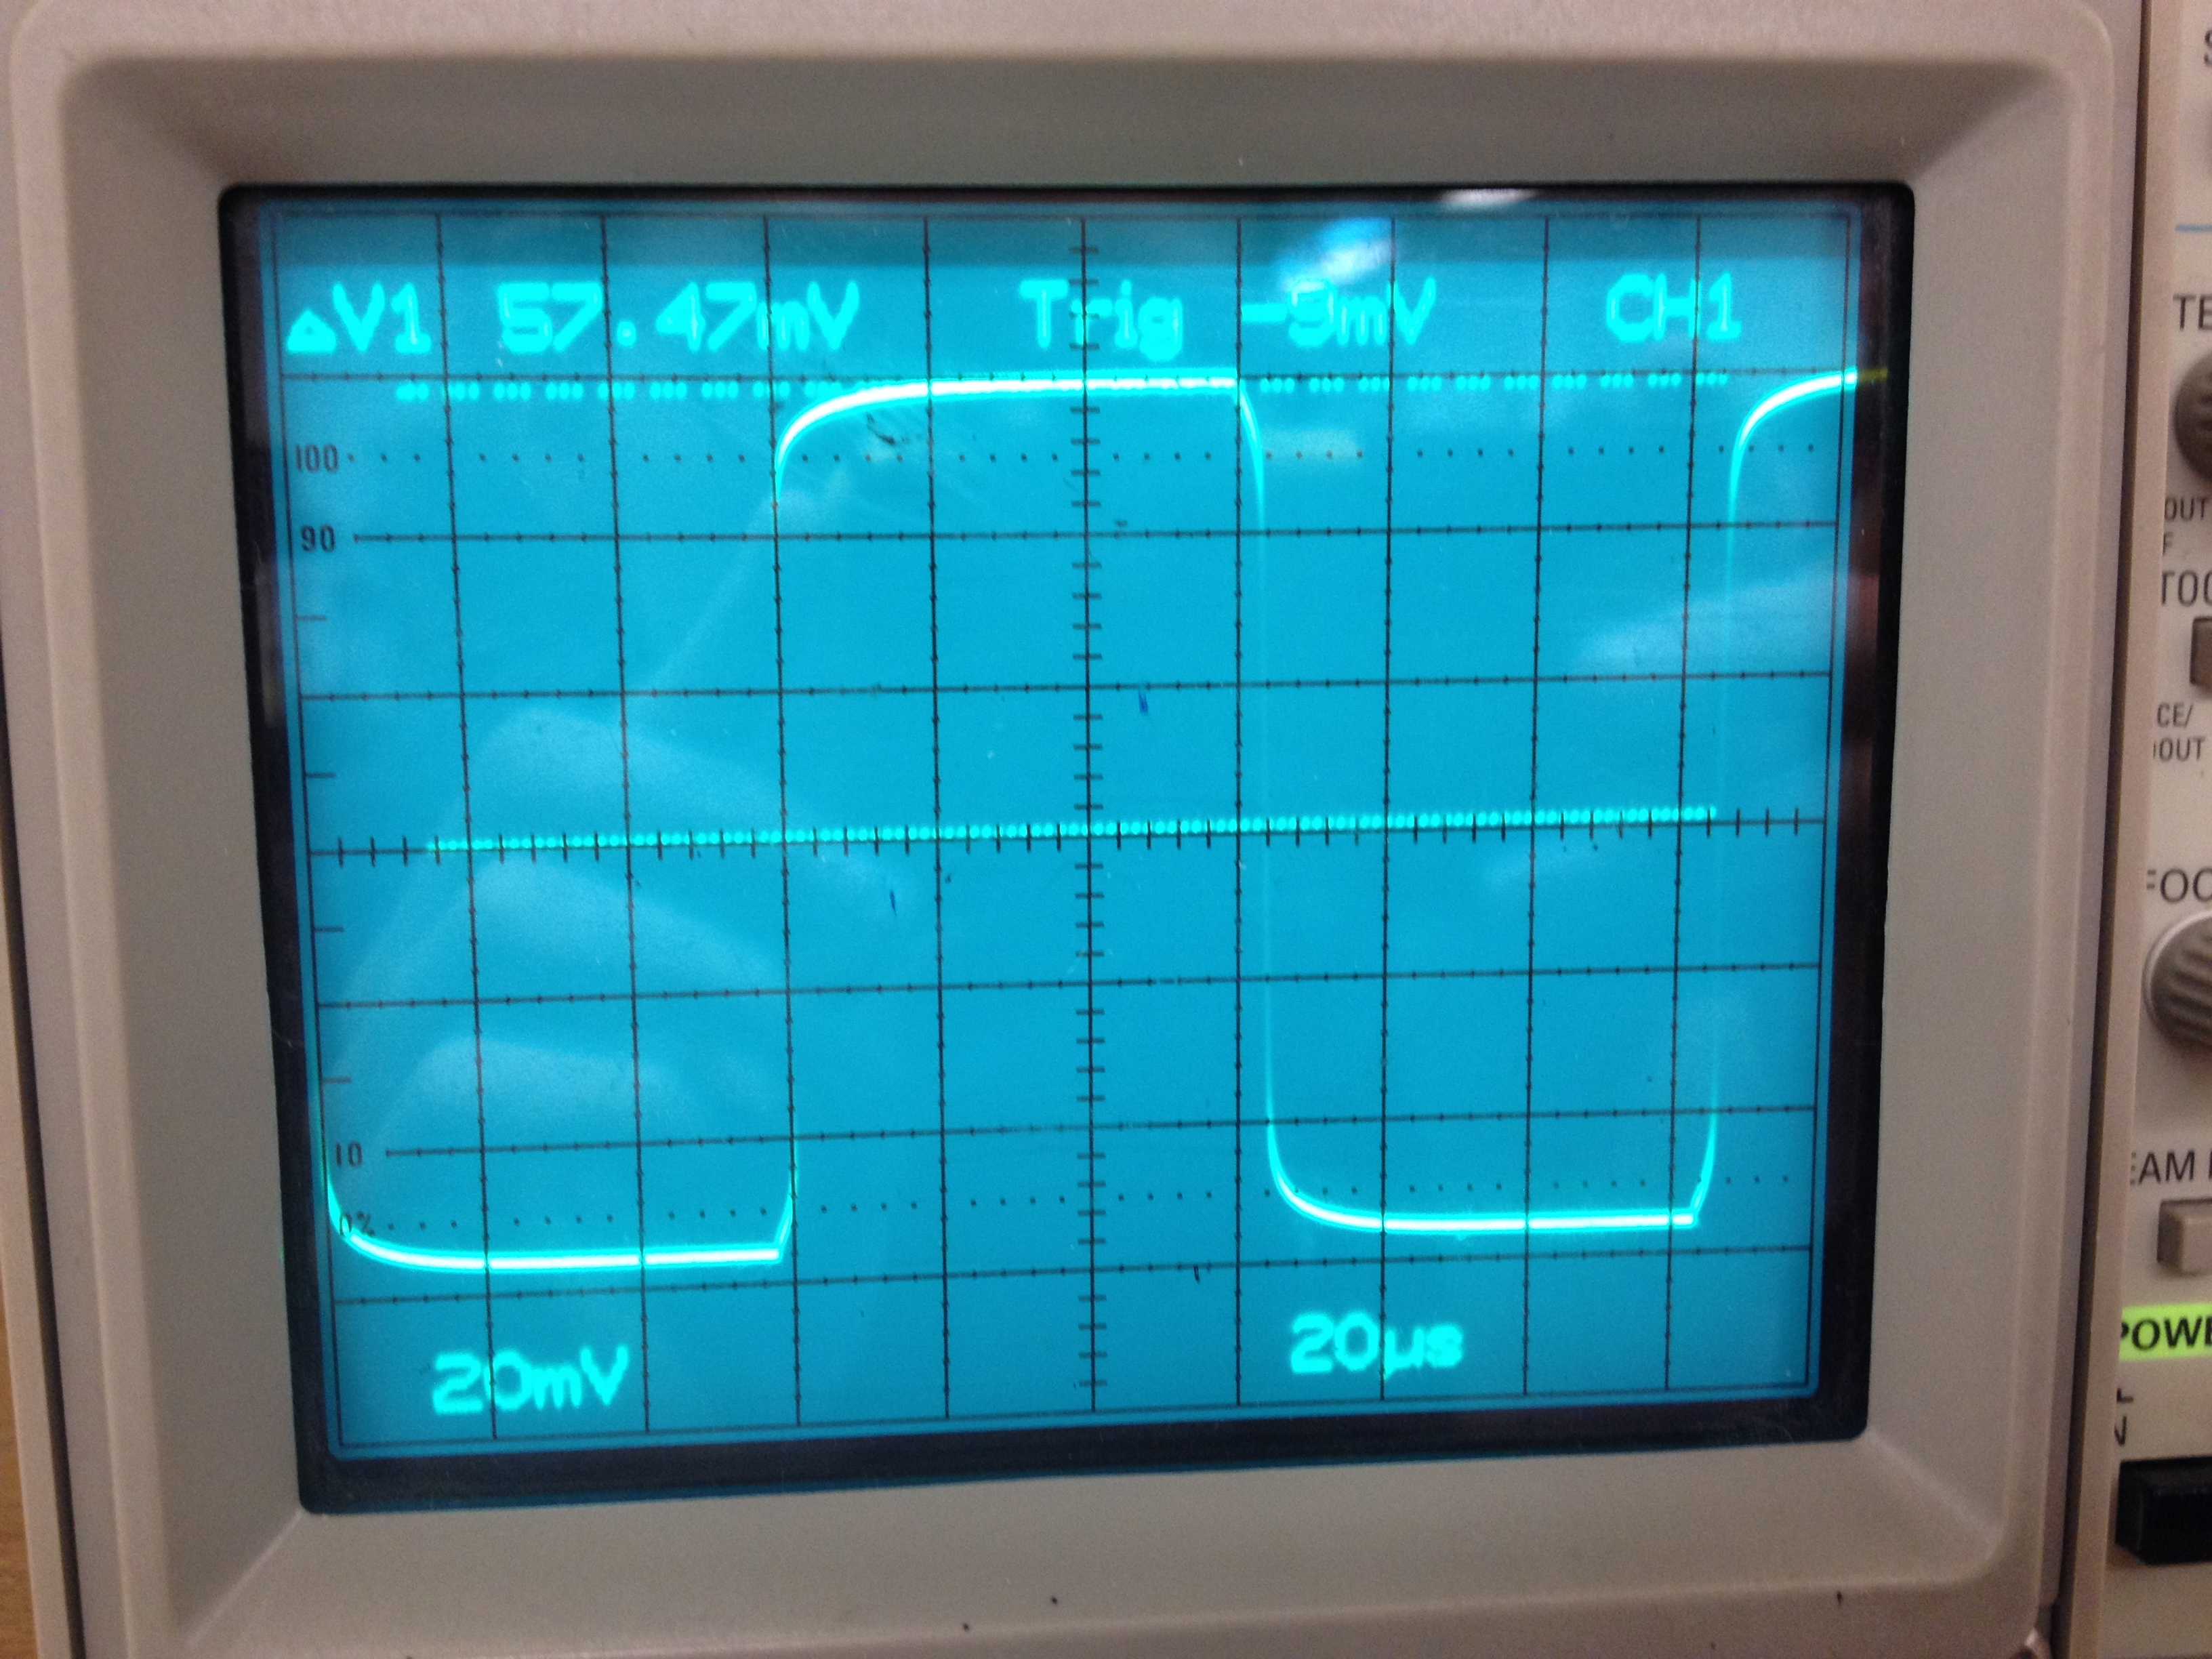
\includegraphics[width=\figwidth, keepaspectratio=true]{lab4/3_7_2.jpg}
\caption{Output waveform of the diode limiter when the input is a 2 $\text{V}_{\text{pp}}$ 8 kHz square wave.}
\label{fig:3_7_2}
\end{figure}

When the input is a triangle wave, the output behaves the same way, except instead of starting as a sin or square wave, it starts looking like an attenuated triangle wave. As the input magnitude increases, the attentuation increases and the output looks more and more like a square wave. The output voltage peak stops increasing at 0.7 V.

\begin{figure}[H]
\centering
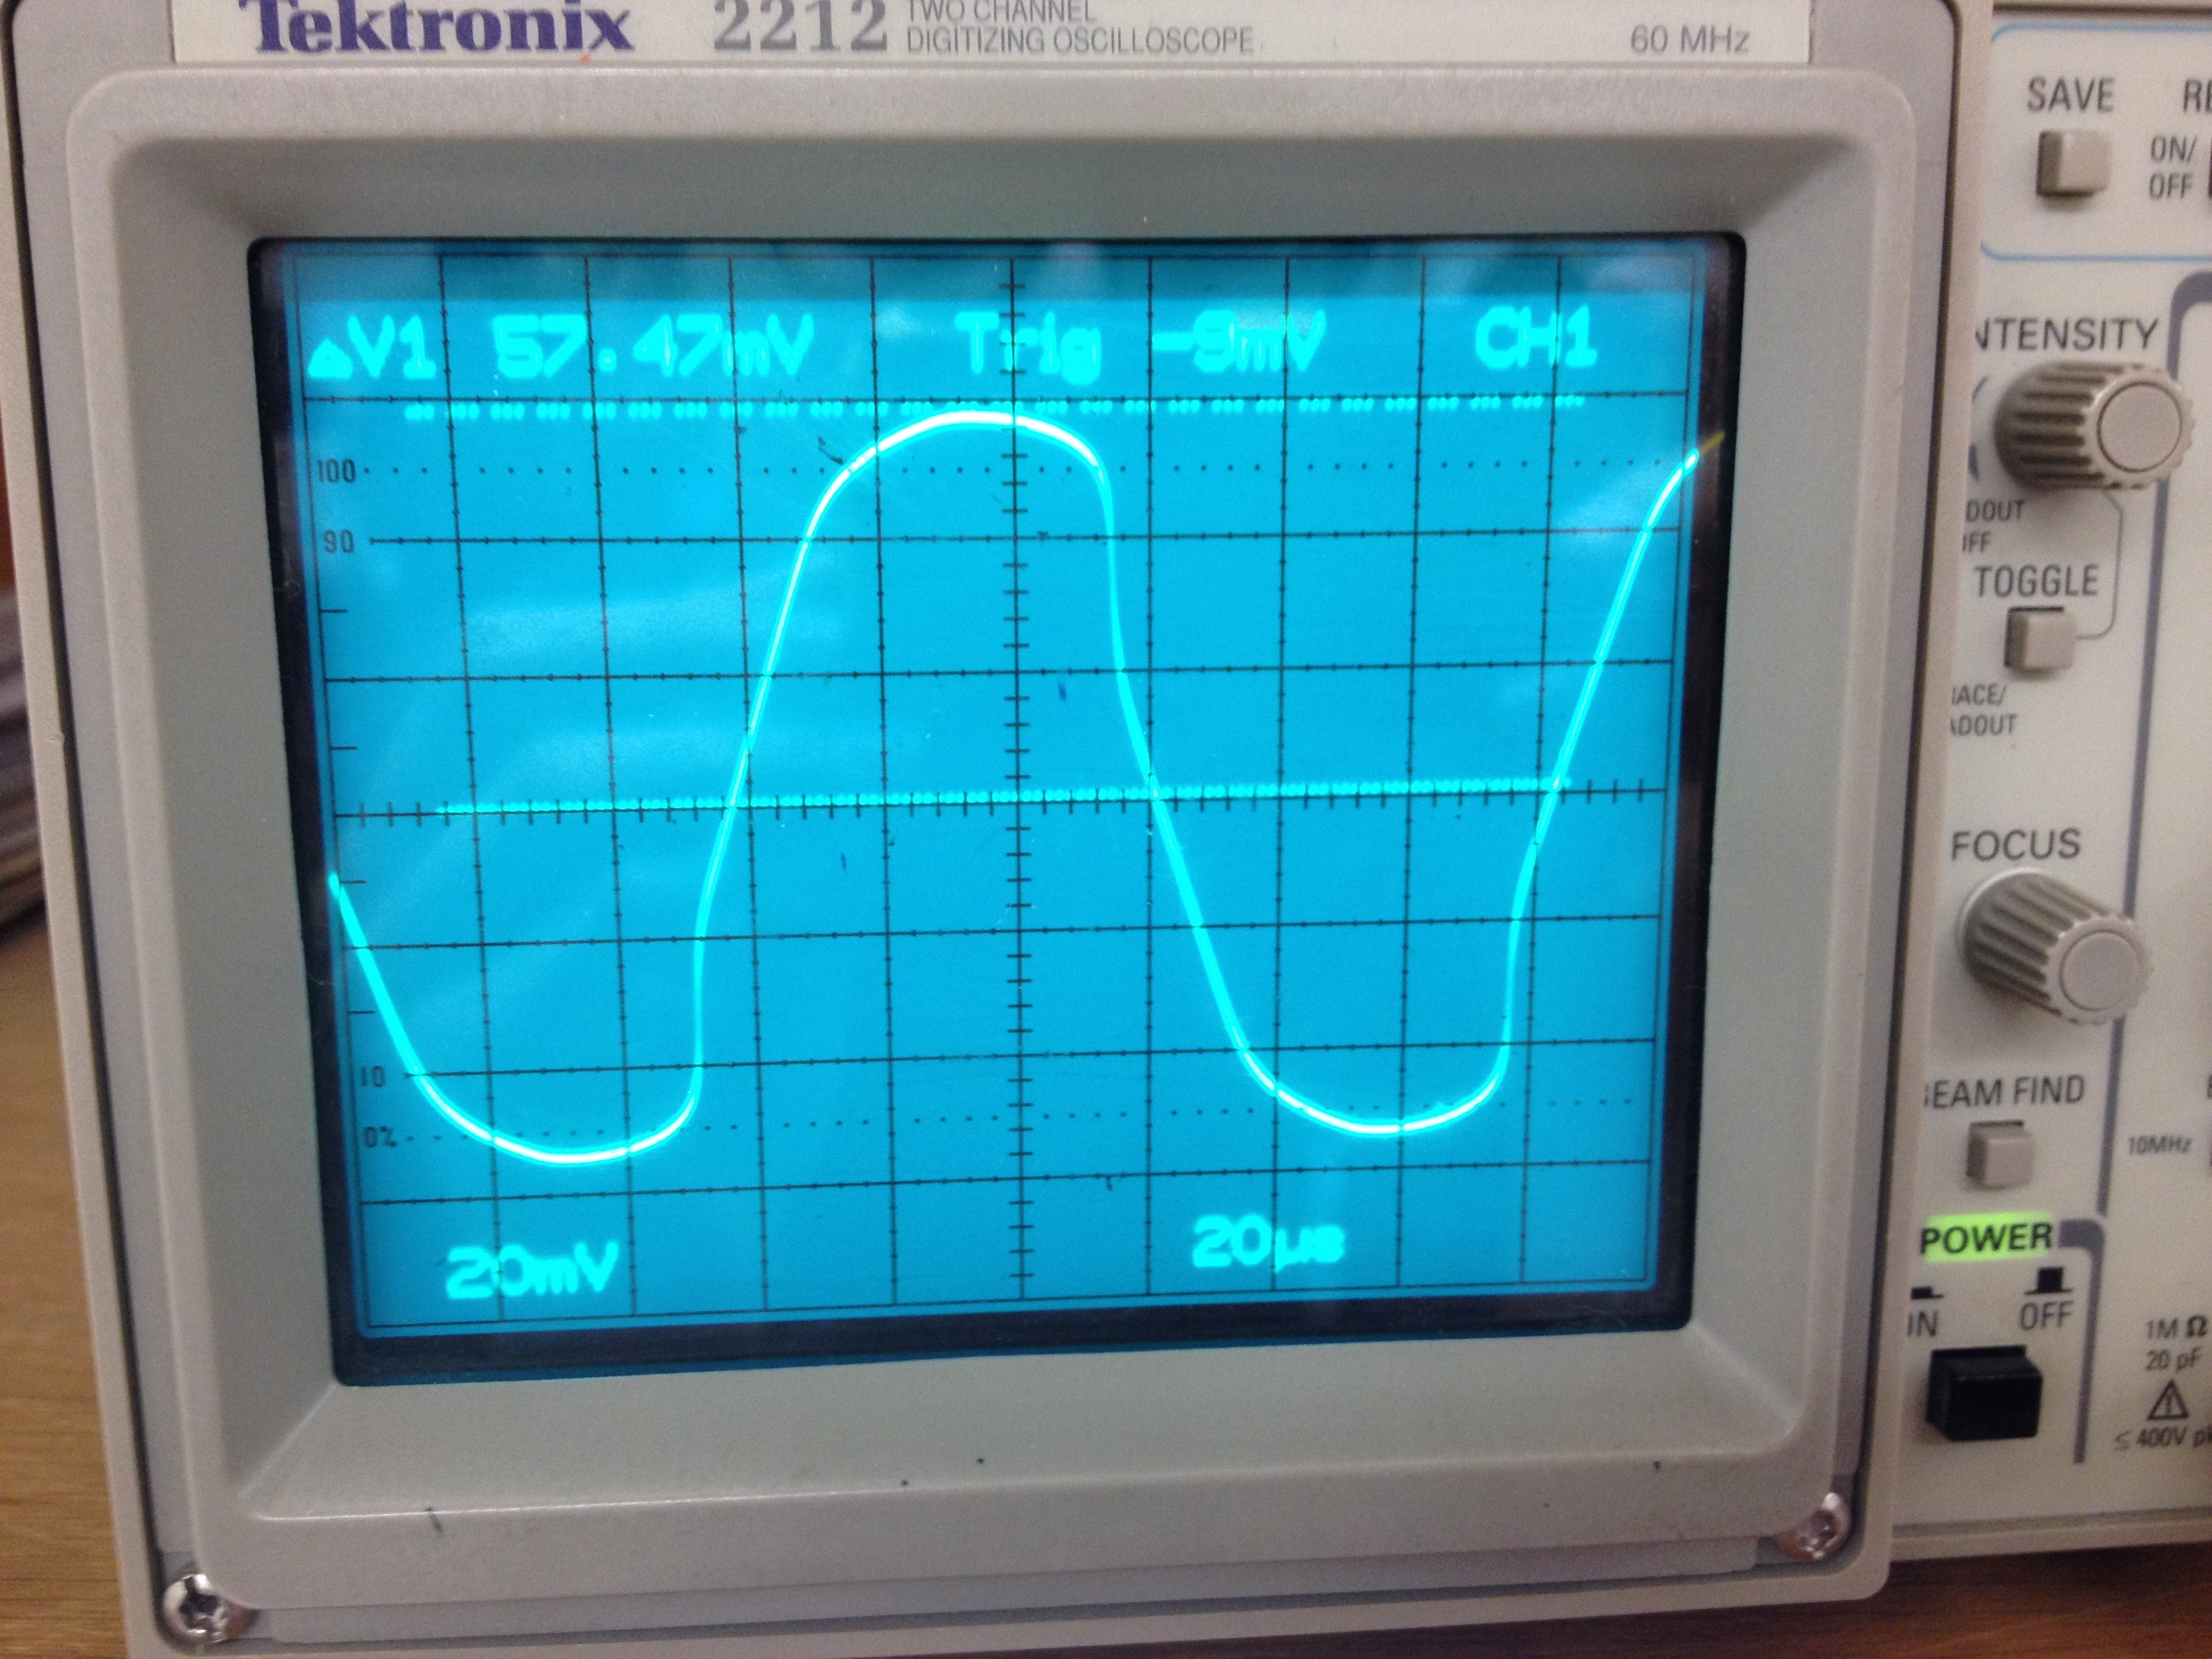
\includegraphics[width=\figwidth, keepaspectratio=true]{lab4/3_7_3.jpg}
\caption{Output waveform of the diode limiter when the input is a 2 $\text{V}_{\text{pp}}$ 8 kHz triangle wave.}
\label{fig:3_7_3}
\end{figure}

The behavior of the circuit remains the same but the output voltage peak is doubled by adding an additional diode to each path of the original circuit.

\begin{table}[ht]
\caption{Output Voltage for Varying Loads} % title of Table
\centering 
    \begin{tabular}{| c | c | c | c |}
    \hline  
    Load (mA) & Resistor Value (k$\Omega$) & $\text{V}_{\text{out}}$ (V) & $ \text{I}_{\text{out}}$ (mA)\\
    \hline
    1 & 5 & 4.93 & 0.89 \\
    50 &.1 & 4.93 & 49 \\
    \hline
    \end{tabular}
    \label{table:voltage_out}
\end{table}

\begin{figure}[H]
\centering
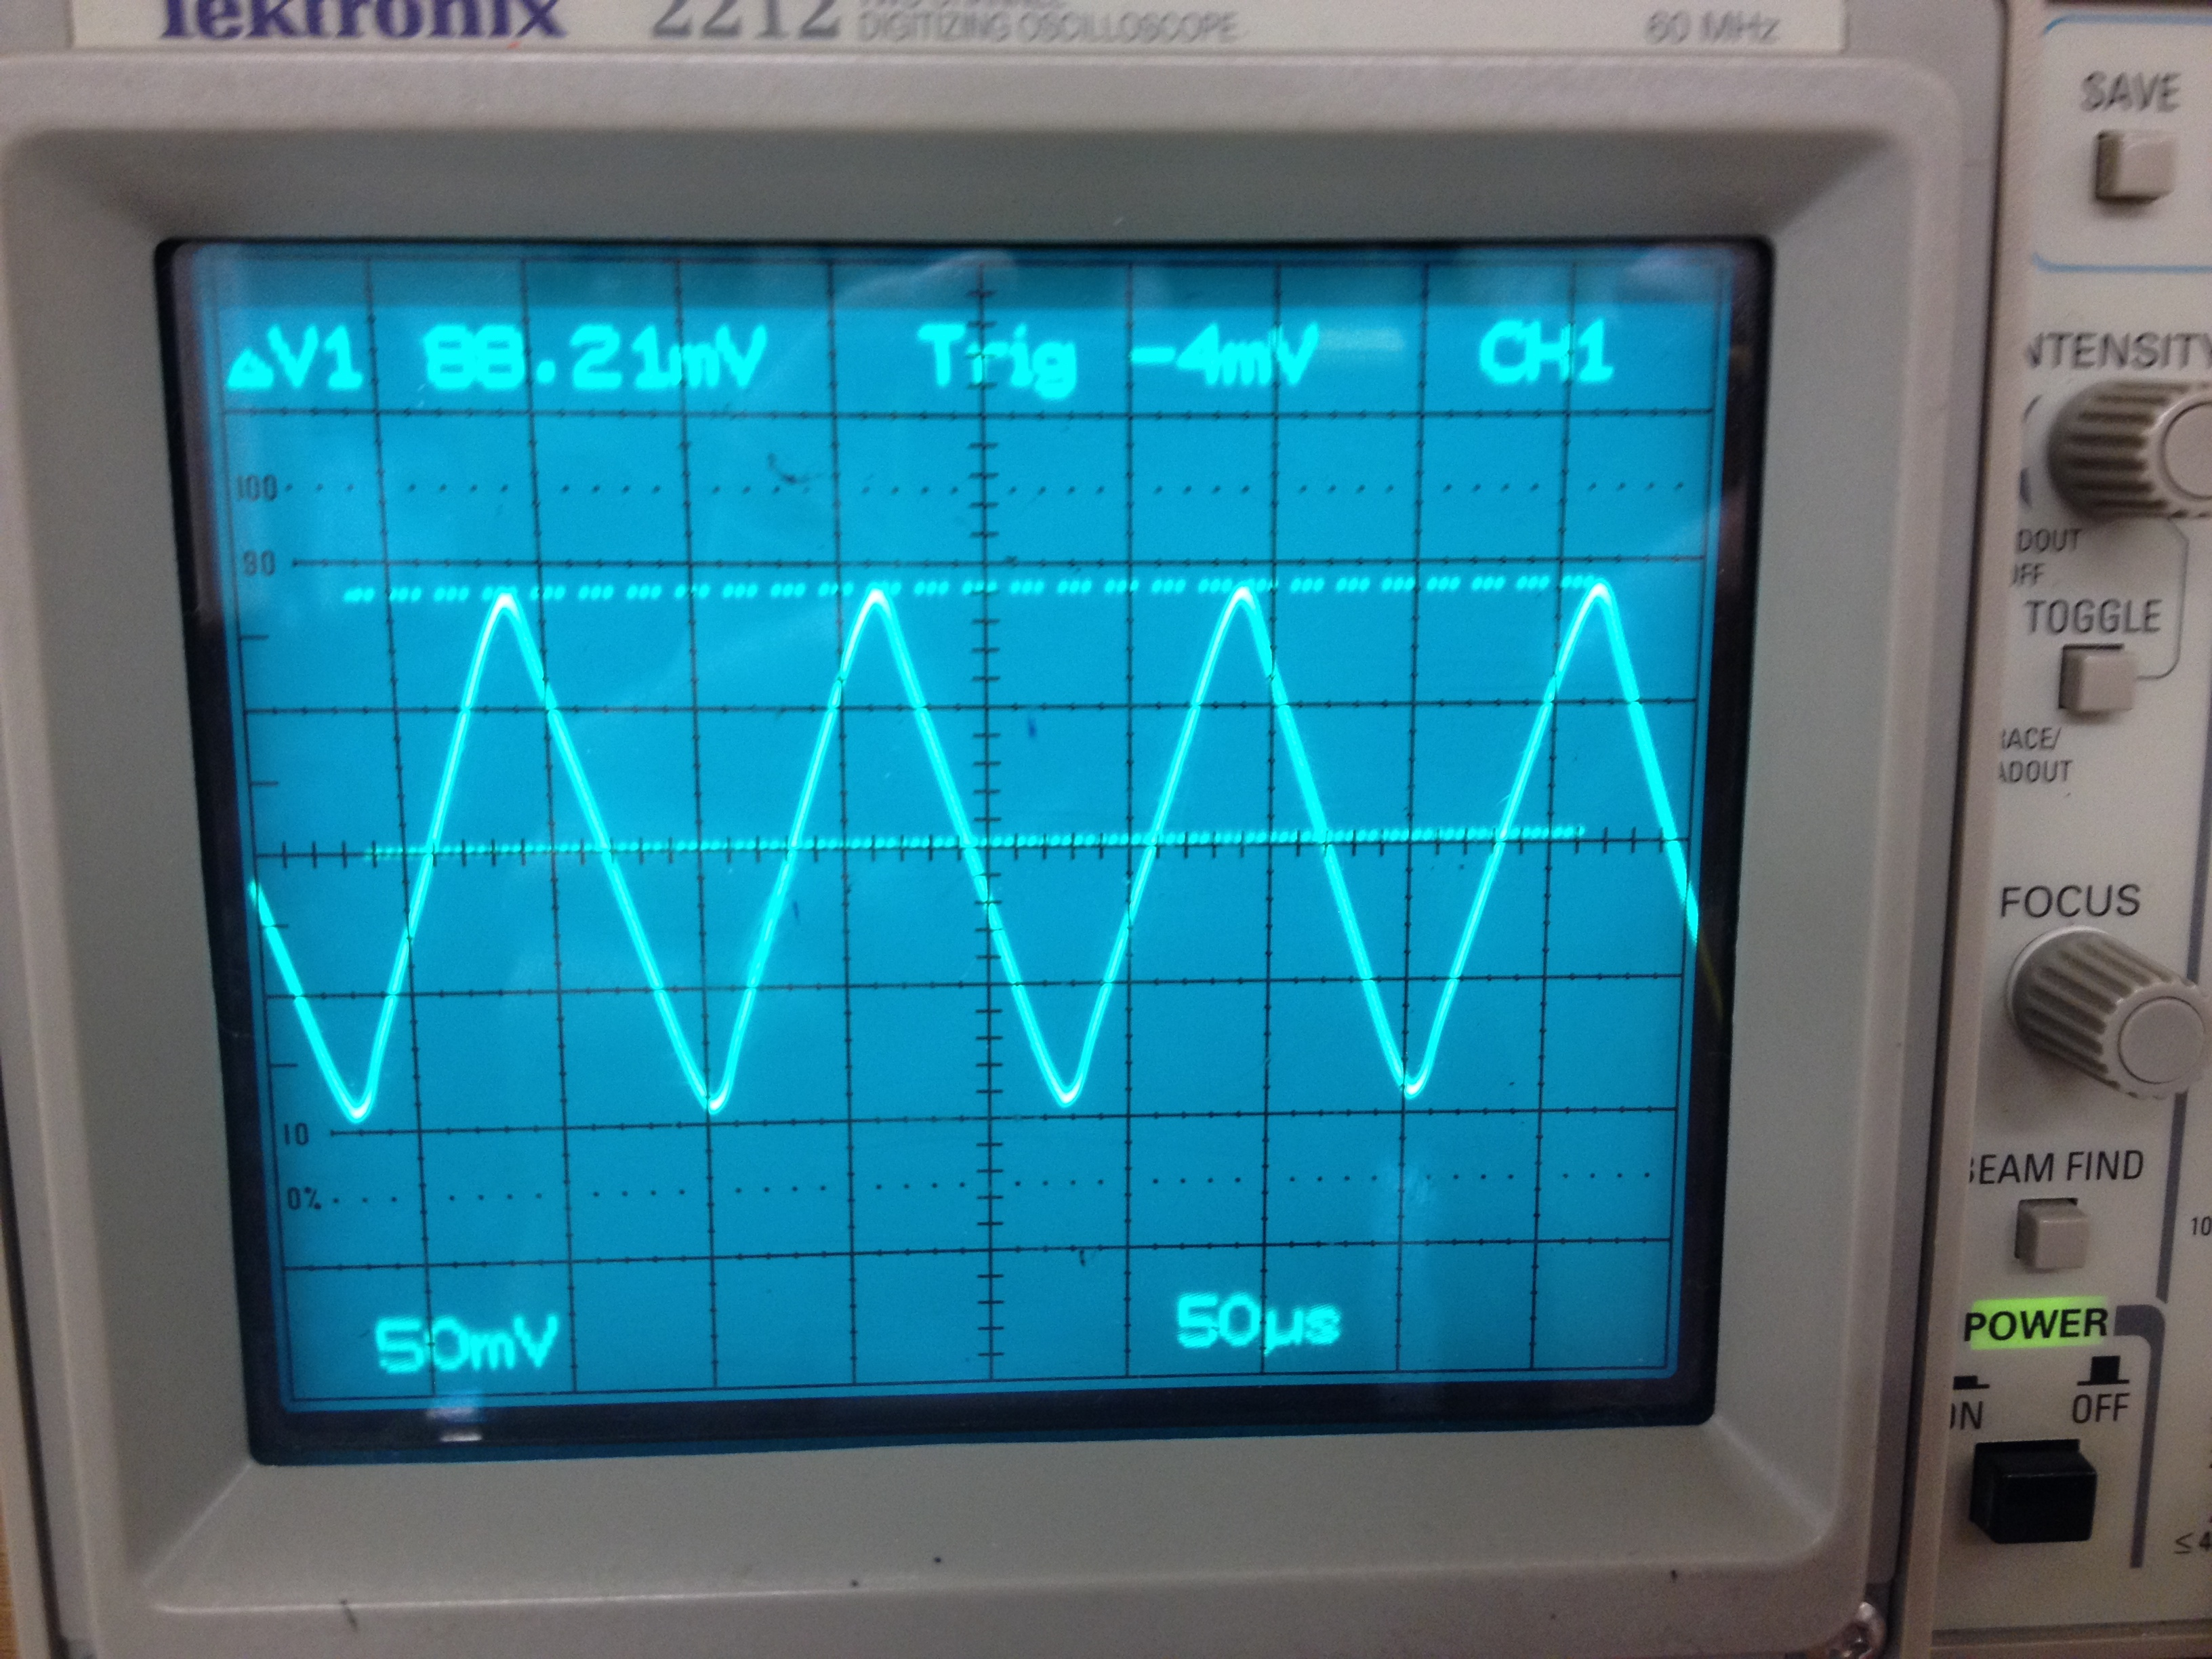
\includegraphics[width=\figwidth, keepaspectratio=true]{lab4/3_7_4.jpg}
\caption{Output waveform of the diode limiter when the input is a 2 $\text{V}_{\text{pp}}$ 8 kHz triangle wave and one additional diode has been added to each path to double the output voltage.}
\label{fig:3_7_4}
\end{figure}

\subsection*{Analysis}

The purpose of this circuit is the limit the output voltage to 0.7 V. This may be used to protect a delicate sensor or other circuit component that cannot be subjected to greater than 0.7 V. Since it has been shown that adding diodes doubles the maximum output voltage, this circuit is not limited to applications that only have a limit of 0.7 V.

Table \ref{table:voltage_out} shows that as the load varies from 1 mA to 50 mA, the output voltage does not change. The only change is in the output current, which increases for increasing load.

\subsection*{Calculations}

Use Ohm's law (V = IR) to calculate the output current based on the measured output voltage value and the known resistor value.
$$
I_{out} = \frac{V_{out}}{R_{load}} = \frac{4.93}{5k} = 0.89\text{ mA}
$$
$$
I_{out} = \frac{V_{out}}{R_{load}} = \frac{4.93}{100} = 49\text{ mA}
$$

\end{document}

% photo 250: 3.2, voltage straight output from the transformer
%photo 252: 3.2, voltage across resistor
%photo 253: 3.3, voltage out of final circuit
%photo 254: 3.2, voltage across resistor of final circuit
%photo 255: 3.2, voltage out of transformer
%photo 256: 3.3, voltage across resistor of the final circuit
%photo 257: 3.4, how to measure delta t
%photo 258: 3.4, how to measure Vr
%photo 259: 3.7, sin, 2Vpp
%photo 260: 3.7, square, 2Vpp
%photo 261: 3.7, triangle, 2Vpp
%photo 262: 3.7, triangle, 2Vpp (we see double output)